% Use the following line _only_ if you're still using LaTeX 2.09.
%\documentstyle[icml2014,epsf,natbib]{article}
% If you rely on Latex2e packages, like most moden people use this:
\documentclass{article}

% use Times
\usepackage{times}
% For figures
\usepackage{graphicx} % more modern
%\usepackage{epsfig} % less modern
\usepackage{subfigure}

% For citations
\usepackage{natbib}

% For algorithms
\usepackage{algorithm}
\usepackage{algorithmic}

% As of 2011, we use the hyperref package to produce hyperlinks in the
% resulting PDF.  If this breaks your system, please commend out the
% following usepackage line and replace \usepackage{icml2014} with
% \usepackage[nohyperref]{icml2014} above.
\usepackage{hyperref}

% Packages hyperref and algorithmic misbehave sometimes.  We can fix
% this with the following command.
\newcommand{\theHalgorithm}{\arabic{algorithm}}

% Employ the following version of the ``usepackage'' statement for
% submitting the draft version of the paper for review.  This will set
% the note in the first column to ``Under review.  Do not distribute.''
\usepackage[accepted]{icml2014}
% Employ this version of the ``usepackage'' statement after the paper has
% been accepted, when creating the final version.  This will set the
% note in the first column to ``Proceedings of the...''
%\usepackage[accepted]{icml2014}


% other packages
\usepackage{../Definitions}
\newcommand{\hmu}{\widehat{\mu}}
\newcommand{\hCcal}{\widehat{\Ccal}}
\newcommand\tl{\widetilde}
\newcommand{\aacomment}[1]{\noindent{\textcolor{blue}{\textbf{\#\#\# AA:} \textsf{#1} \#\#\#}}}

% \newcommand{\bm}{\mathbf}

\newcommand{\sk}[1]{\noindent{\textcolor{cyan}{\{{\bf SK:} \em #1\}}}}
\newcommand{\djh}[1]{\noindent{\textcolor{blue}{\textbf{\#\#\# DJH:} \textsf{#1} \#\#\#}}}
\newcommand{\aacomment}[1]{\noindent{\textcolor{blue}{\textbf{\#\#\# AA:} \textsf{#1} \#\#\#}}}
\newcommand{\rg}[1]{\noindent{\textcolor{blue}{\textbf{\#\#\# RG:} \textsf{#1} \#\#\#}}}
\DeclareMathOperator{\Ber}{Ber}

\def\tcr{\textcolor{red}}
\def\tcb{\textcolor{blue}}
\def\tha{{\mbox{\tiny th}}}
\def\Ibb{{\mathbb I}}

\DeclareMathOperator{\thres}{Thres}
\DeclareMathOperator{\Var}{Var}
\DeclareMathOperator\Diag{Diag}

\DeclareMathOperator{\polylog}{polylog}
% \DeclareMathOperator*{\argmin}{arg\,min}
% \DeclareMathOperator*{\argmax}{arg\,max}
\newcommand\E{\mathbb{E}}
\newcommand\R{\mathbb{R}}
\renewcommand\t{{\scriptscriptstyle\top}}
\newcommand\myvec[1]{\underline{#1}}
\newcommand\prior[1]{\ensuremath{\myvec{\pi_{#1}}}}
\newcommand\com[1]{\ensuremath{\myvec{o_{#1}}}}
\newcommand\e[1]{\ensuremath{\myvec{e_{#1}}}}
%\newcommand\ind[1]{\ensuremath{\mathds{1}_{\{#1\}}}}
\renewcommand\inner[1]{\ensuremath{\left<#1\right>}}
\newcommand\norm[1]{\left\|#1\right\|}
%\newcommand\bigO{\mathbb{O}}
\newcommand\bigO{O}
\newcommand\tlO{\tilde{\bigO}}
\def\t{{\scriptscriptstyle\top}}
\def\tl{\widetilde}
\def\h{\widehat}
\def\halpha{\widehat{\alpha}}
\def\tT{\tilde{T}}
\newcommand\dotp[1]{\langle #1 \rangle}
\def\Sig{\varSigma}
\def\tree{\mathcal{T}}
\def\hp{\hphantom}
\def\eps{\epsilon}
\def\veps{\varepsilon}
\def\simiid{{\overset{iid}{\sim}}}
\def\Pbb{{\mathbb P}}
\DeclareMathOperator{\poly}{poly}
\DeclareMathOperator{\Gammadist}{GammaCDF}
\def\Ac{{\cal A}}
\def\Bc{{\cal B}}
\def\bfd{{\mathbf d}}
\def\bfm{{\mathbf m}}
\def\Cc{{\cal C}}
\DeclareMathOperator{\Span}{span}
\renewcommand\th[1]{\ensuremath{\theta_{#1}}}
\newcommand\hth[1]{\ensuremath{\hat{\theta}_{#1}}}
\newcommand\teps{\ensuremath{\tilde{\eps}}}
\newcommand\hv{\ensuremath{\hat{v}}}
\newcommand\hlambda{\ensuremath{\hat{\lambda}}}
\newcommand\lambdamin{\ensuremath{\lambda_{\min}}}
\newcommand\lambdamax{\ensuremath{\lambda_{\max}}}
\newcommand\deflate{\mathcal{E}}
 \newcommand\tlambdamin{\ensuremath{\tilde{\lambda}_{\min}}}

\DeclareMathOperator{\eqa}{\overset{(a)}{=}}


\newcommand{\red}[1]{\textcolor{red}{#1}}
%\DeclareMathOperator{\diag}{diag}
\DeclareMathOperator{\range}{range}
%\DeclareMathOperator{\rank}{rank}
\DeclareMathOperator{\sign}{sign}
\DeclareMathOperator{\Pairs}{Pairs}
\DeclareMathOperator{\Triples}{T}

\newcommand\Dir{\operatorname{Dir}}

% environments
%\newtheorem{theorem}{Theorem}[section]
%\newtheorem*{namedtheorem}{\theoremname}
%\newcommand{\theoremname}{testing}
%\newenvironment{named}[1]{ \renewcommand{\theoremname}{#1} \begin{namedtheorem}} {\end{namedtheorem}}
%\newtheorem{thm}[theorem]{Theorem}
%\newtheorem{lemma}[theorem]{Lemma}
%\newtheorem{lem}[theorem]{Lemma}
%\newtheorem*{claim}{Claim}
%\newtheorem{clm}[theorem]{Claim}
%\newtheorem{proposition}[theorem]{Proposition}
%\newtheorem{prop}[theorem]{Proposition}
%\newtheorem{fact}[theorem]{Fact}
%\newtheorem{res}{Restriction}
%\newtheorem{observation}{Observation}
%\newtheorem{corollary}[theorem]{Corollary}
%\newtheorem{cor}[theorem]{Corollary}
%\theoremstyle{definition}
%\newtheorem{definition}[theorem]{Definition}
%\newtheorem{defn}[theorem]{Definition}

\newcommand{\bp}{\begin{psfrags}}
\newcommand{\ep}{\end{psfrags}}
\newcommand{\bprfof}{\begin{proof_of}}
\newcommand{\eprfof}{\end{proof_of}}
\newcommand{\bprf}{\begin{myproof}}
\newcommand{\eprf}{\end{myproof}}

\newenvironment{myproof}{\noindent{\em Proof:} \hspace*{1em}}{
    \hspace*{\fill} $\Box$ }
\newenvironment{proof_of}[1]{\noindent {\em Proof of #1: }}{\hspace*{\fill} $\Box$ }

\def\viz{{viz.,\ \/}}
\def\Ebb{{\mathbb E}}
\def\nn{\nonumber}
\def\beq{\begin{equation}}
\def\eeq{\end{equation}\noindent}
\def\beqn{\begin{eqnarray}}
\def\eeqn{\end{eqnarray} \noindent}
\def\beqnn{  \begin{eqnarray*}}
\def\eeqnn{\end{eqnarray*}  \noindent}
\def\bcase{  \begin{numcases}}
\def\ecase{\end{numcases}   \noindent}

\usepackage{tikz}
\usetikzlibrary{calc}
\usepackage{exscale,relsize}
\usepackage{enumitem}

\usepackage{color}
\newcommand{\Le}[1]{{\color{red}{\bf\sf [note: #1]}}}
\newcommand{\bodai}[1]{{\color{violet}{\bf\sf [Dai remark: #1]}}}
\newcommand{\boxie}[1]{{\color{green}{\bf\sf [Bo Xie comment: #1]}}}

% The \icmltitle you define below is probably too long as a header.
% Therefore, a short form for the running title is supplied here:
\icmltitlerunning{Nonparametric Estimation of Multi-view Latent Variable Models}

\begin{document}

\twocolumn[
\icmltitle{Nonparametric Estimation of Multi-View Latent Variable Models}

% It is OKAY to include author information, even for blind
% submissions: the style file will automatically remove it for you
% unless you've provided the [accepted] option to the icml2014
% package.
\vskip -0.2in

\icmlauthor{Le Song}{lsong@cc.gatech.edu}
\icmladdress{Georgia Institute of Technology,
            Atlanta, GA 30345 USA}
\vskip -0.05in            
\icmlauthor{Animashree Anandkumar}{a.anandkumar@uci.edu}
\icmladdress{University of California, Irvine, CA 92697, USA}
\vskip -0.05in
\icmlauthor{Bo Dai, Bo Xie}{bdai6,bxie33@gatech.edu}
\icmladdress{Georgia Institute of Technology, Atlanta, GA 30345 USA}


% You may provide any keywords that you
% find helpful for describing your paper; these are used to populate
% the "keywords" metadata in the PDF but will not be shown in the document
% \icmlkeywords{Kernel Methods, Latent Variable Models, Spectral Algorithms}

\vskip 0.1in
]

\begin{abstract}
		Spectral methods have greatly advanced the estimation of latent variable models, generating a sequence of novel and efficient algorithms with strong theoretical guarantees.
		However, current spectral algorithms are largely restricted to mixtures of discrete or Gaussian distributions. In this paper, we propose a kernel method for learning multi-view latent variable models, allowing each mixture component to be nonparametric and learned from data in an \emph{unsupervised} fashion. The key idea of our method is to embed the joint distribution of a multi-view latent variable model into a reproducing kernel Hilbert space, and then the latent parameters are recovered using a robust tensor power method. We establish that the  sample complexity for the proposed method is quadratic in the number of latent components and is a low order polynomial in the other relevant parameters. Thus, our nonparametric tensor approach to learning latent variable models enjoys good sample and computational efficiencies. As a special case of our framework, we also obtain a first \emph{unsupervised} conditional density estimator of the kind with provable guarantees. 	In both synthetic and real world 
datasets, the nonparametric tensor power method compares favorably to EM algorithm and other spectral algorithms.
\end{abstract}

\vspace{-5mm}
\section{Introduction} \label{sec:intro}
\vspace{-2mm}

\setlength{\abovedisplayskip}{4pt}
\setlength{\abovedisplayshortskip}{1pt}
\setlength{\belowdisplayskip}{4pt}
\setlength{\belowdisplayshortskip}{1pt}
\setlength{\jot}{3pt}

%\setlength{\floatsep}{1ex}
\setlength{\textfloatsep}{3ex}

% Latent variable models have been used to address various machine learning
% problems, ranging from modeling temporal dynamics, to text document analysis and to social network analysis~\citep{RabJua86,Clark90,HofRafHan02,BleNgJor03}.
Recently, there is a surge of interest in designing spectral algorithms for estimating the parameters of latent variable models~\citep{HsuKakZha09,SonBooSidGorSmo10,ParSonXin11,SonParXin11,FosRodUng12,AnandkumarEtal:tensor12, AnandkumarEtal:twosvd12}. Compared to the Expectation-Maximization (EM) algorithm \citep{DemLaiRub77} traditionally used for this task, spectral algorithms are better in terms of their computational efficiency and provable guarantees.
However, current spectral algorithms are largely restricted to mixture
of discrete or Gaussian distributions, e.g.~\citep{AnandkumarEtal:tensor12,HsuKak13}. When the mixture components are distributions other than these standard distributions, the theoretical guarantees for these algorithms are no longer applicable, and their empirical performance can be very poor.

We propose a kernel method for obtaining sufficient statistics of a multi-view latent variable model (for $\ell\geq 3$),
\begin{align}
  \PP\rbr{\{X_t\}_{t \in [\ell]}}=\sum\nolimits_{h \in [k]} \PP(h) \cdot \prod\nolimits_{t \in [\ell]} \PP(X_t|h),
  \label{eq:multiview_model}
\end{align}
given samples only from the observed variables $\{X_t\}_{t \in [\ell]}$, but \emph{not} the hidden variable $H$. These statistics allow us to answer integral query, $\int_{\Xcal} f(x_t)\, d \PP(x_t|h)$, for functions $f$ from a reproducing kernel Hilbert space (RKHS) \emph{without} the need to assume any parametric form for the involved latent component $\PP(X_t|h)$ (we call this setting ``\emph{unsupervised}''). Note that this is a very challenging problem, since we do not have samples to directly estimate $\PP(X_t|h)$. Hence traditional kernel density estimator does not apply. Furthermore, the nonparametric form of $\PP(X_t|h)$ renders previous spectral methods inapplicable.

Our solution is to embed the distribution of the observed variables in such a model into a reproducing kernel Hilbert space, and exploit tensor decomposition of the embedded distribution (or covariance operators)
to recover the unobserved embedding $\mu_{X_t|h}=\int_{\Xcal} \phi(x)\, d\PP(x|h)$ of the mixture components. The key computation of our algorithm involves a kernel singular value decomposition of the two-view covariance operator, followed by a robust tensor power method on the three-view covariance operator. These standard matrix operations makes the algorithm very efficient and easy to deploy.

Although kernel methods have been previously applied to learning latent variable models, none of them can provably recover the exact latent component $\PP(X_t|h)$ or its sufficient statitiscs to support integral query on this distribution. For instance, \citet{SonBooSidGorSmo10,SonParXin11, SonDai13}~estimated an (unknown) invertible transformation of the sufficient statistics of the latent component $\PP(X_t|h)$, and only supported integral query associated with the distribution of the observed variables. \citet{SgoJanPetSch13}~used kernel independence measure to cluster data points, and treated each cluster as a latent component. Besides computational issues, it is also difficult to provide theoretical guarantees to such an approach since the clustering step only finds a local minimum. \citet{BenChaHun09} designed an EM-like algorithm for learning the conditional densities in latent variable models. This algorithm alternates between the E-step, proportional assignment of data points to components, and the M-step, kernel 
density estimation based on weighted data points. Similarly, theoretical analysis of such a local search heurstic is difficult.

The kernel algorithm proposed in this paper is also significantly more general than the previous spectral algorithms which work only for distributions with parametric assumptions~\cite{AnandkumarEtal:tensor12,HsuKak13}. In fact, when we use the delta kernel, our algorithm recovers the previous algorithm of~\citet{AnandkumarEtal:tensor12} for discrete mixture components as a special case. When we use universal kernels, such as the Gaussian RBF kernel, our algorithm can recover Gaussian mixture components as well as mixture components with other distributions. In this sense, our work also provides a unifying framework for previous spectral algorithms. We prove sample complexity bounds for the nonparametric tensor power method and show that it is both computational and sample efficient. As a special case of our framework, we also obtain a first \emph{unsupervised} conditional density estimator of the kind with provable guarantees. Furthermore, our approach can also be generalized to other latent variable 
learning tasks such as independent component analysis and latent variable models with Dirichlet priors.
% establish  that the sample complexity is quadratic in the number of latent components, and is a low order polynomial in the other relevant parameters such as the lower bound on mixing weights. Thus, we propose a computational and sample efficient nonparametric approach to learning
% latent variable models.

Experimentally, we corroborate our theoretical results by comparing our algorithm to the EM algorithm and previous spectral algorithms. We show that when the model assumptions are correct for the EM algorithm and previous spectral algorithms, our algorithm converges in terms of estimation error to these competitors. In the opposite cases when the model assumptions are incorrect, our algorithm is able to adapt to the nonparametric mixture components and beating alternatives by a very large margin.

%%%%%%%%%%%%%%%%%%%%%%%%%%%%%%%%%%%%%%%%%%%%%%%%%%%%%%%%%%%%%%%%%%%%%%%%%%%%%%%%%%%%%%%%%%%%%%
\vspace{-3mm}
\section{Notation}
\vspace{-2mm}
%%%%%%%%%%%%%%%%%%%%%%%%%%%%%%%%%%%%%%%%%%%%%%%%%%%%%%%%%%%%%%%%%%%%%%%%%%%%%%%%%%%%%%%%%%%%%%

We  denote by $X$ a random variable with domain $\Xcal$,
and refer to instantiations of $X$ by the lower case character, $x$.
We endow $\Xcal$ with some $\sigma$-algebra $\Ascr$ and denote a distributions (with respect to $\Ascr$) on $\Xcal$ by $\PP(X)$. For the multi-view model in equation~\eq{eq:multiview_model}, we also deal with multiple random variables, $X_1, X_2, \ldots, X_{\ell}$, with joint distribution $\PP(X_1,X_2,\ldots,X_{\ell})$. For simplicity of notation, we assume that the domains of all $X_t, t \in [\ell]$ are the same, but the methodology applies to the cases where they have different domains. Furthermore, we denote by $H$ a hidden variable with domain $\Hcal$ and distribution $\PP(H)$.

A \emph{reproducing kernel Hilbert space (RKHS)} $\Fcal$ on $\Xcal$ with a kernel $\kappa(x,x')$ is a Hilbert space of
functions $f(\cdot):\Xcal \mapsto \RR$ with inner product $\inner{\cdot}{\cdot}_{\Fcal}$. Its element $\kappa(x,\cdot)$ satisfies the reproducing property:
$\inner{f(\cdot)}{\kappa(x, \cdot)}_{\Fcal} = f(x)$, and consequently, $\inner{\kappa(x,\cdot)}{\kappa(x', \cdot)}_{\Fcal} = \kappa(x,x')$,
meaning that we can view the evaluation of a function $f$ at any point $x\in\Xcal$ as an inner product. Alternatively, $\kappa(x,\cdot)$ can  be viewed as an implicit feature map $\phi(x)$ where $\kappa(x,x')=\inner{\phi(x)}{\phi(x')}_{\Fcal}$.
In this paper, we will focus on $\Xcal=\RR^d$, and the \emph{normalized} Gaussian RBF kernel
\begin{align}
\kappa(x,x') = \exp(- \nbr{x-x'}^2 / (2 s^2)) / (\sqrt{2\pi} s^d). \label{eq:normalizedrbf}
\end{align}
But kernel functions have also been defined on
graphs, time series, dynamical systems, images and other structured
objects \, \cite{SchTsuVer04}. Thus the methodology presented below can be readily generalized to a diverse range of data types as long as kernel functions are defined.
% Similarly, we denote by $\Gcal$ an RKHS on $\Hcal$ with kernel $l(h,h')$, and by $\psi(h)$ the corresponding feature map.

% Furthermore, we let $h \in [k]$ be a discrete random variable with $P(h =
% j) = r_j$ for all $j \in [k]$.
%
% We denote by $X$ a random variable with domain $\Xcal$ and distribution $P(X)$, and refer to instantiations of $X$ by the lower case character, $x$.
% We  focus on continuous domains, and denote the corresponding density by $p(X)$. We  also deal with multiple random variables, $X_1, X_2, \ldots, X_{\ell}$, with joint distribution $P(X_1,X_2,\ldots,X_{\ell})$. For simplicity of notation, we assume that the domain of all $X_t, t \in [\ell]$ also be $\Xcal$, but the methodology applies to the cases where they have different domains. Furthermore, we let $H \in [k]$ be a discrete random variable with $P(H =
% j) = r_j$ for all $j \in [k]$.


\vspace{-3mm}
\section{Kernel Embedding of Distributions}
\label{sec:embedding}
\vspace{-2mm}

Kernel embeddings of distributions are \emph{implicit} mappings of distributions into potentially \emph{infinite} dimensional RKHS.
% \footnote{By ``implicit'', we mean that we do not need to explicitly construct the feature spaces, and the actual computations boil down to kernel matrix operations.}
The kernel embedding approach represents a distribution by an element in the RKHS associated with a kernel function \, \cite{SmoGreSonSch07},
\begin{align}
  \mu_{X} \, := \, \EE_{X} \sbr{\phi(X)} \, = \, \int_{\Xcal} \phi(x) \, d\PP(x),  \label{eq:embedding}
\end{align}
where the distribution is mapped to its expected feature map,~\ie,~to a point in a potentially infinite-dimensional and implicit feature space.
By the reproducing property of an RKHS, the kernel embedding is a sufficient statistic for integral query $\forall f\in\Fcal$,~\ie,~
$
  \int_{\Xcal} f(x)\, d\PP(x)  = \inner{\mu_{X}}{f}_{\Fcal}.
$
Kernel embedding of distributions has rich representational power. The mapping is injective for characteristic kernels~\cite{SriGreFukLanetal08}. That is, if two distributions, $\PP(X)$ and $\QQ(X)$, are different, they are mapped to two distinct points in the RKHS. For domain $\RR^d$, many commonly used kernels are characteristic, such as the normalized Gaussian RBF kernel.

Kernel embeddings can be readily generalized to joint distributions of two or more variables using tensor product feature maps. We can embed the joint distribution of two variables $X_1$ and $X_2$ into a tensor product feature space $\Fcal\times \Fcal$ by
$
    \Ccal_{X_1X_2} :=
    \int_{\Xcal \times \Xcal} \phi(x_1) \otimes \phi(x_2) \, d\PP(x_1, x_2),
$
% \begin{align*}
%     \Ccal_{X_1X_2} \, &:= \, \EE_{X_1X_2}[\phi(X_1)\otimes \phi(X_2)] \\
%     \, &= \, \int_{\Xcal \times \Xcal} \phi(x_1) \otimes \phi(x_2) \, d\PP(x_1, x_2),
% \end{align*}
where the reproducing kernel for the tensor product features satisfies
$
	\inner{\phi(x_1)\otimes \phi(x_2) }{\phi(x_1')\otimes \phi(x_2') }_{\Fcal\times \Fcal} \, = \,  \kappa(x_1,x_1')\,\kappa(x_2,x_2').
$
By analogy, we can also define $\Ccal_{X_1X_2X_3} := \EE_{X_1X_2X_3}[\phi(X_1)\otimes\phi(X_2)\otimes \phi(X_3)]$.

Given a sample $\Dcal_{X} = \cbr{x^1, \ldots, x^m}$ of size $m$ drawn~\iid~from $\PP(X)$, the empirical kernel embedding can be estimated simply as
$\hmu_{X} = \frac{1}{m} \sum\nolimits_{i=1}^m \phi(x^i)$ with an error $\|\hmu_X - \mu_X \|_{\Fcal}$ scaling as $O_p(m^{-\frac{1}{2}})$~\cite{SmoGreSonSch07}.
Similarly, $\Ccal_{X_1X_2}$ and $\Ccal_{X_1X_2X_3}$ can be estimated as
$
 \widehat \Ccal_{X_1X_2} =\frac{1}{m}\sum\nolimits_{i=1}^m \phi(x_1^i) \otimes \phi(x_2^i)
$, and
$\widehat \Ccal_{X_{1:3}} = \frac{1}{m} \sum_{i = 1}^m \phi(x_1^i) \otimes \phi(x_2^i) \otimes \phi(x_3^i)$ respectively.
Note that we never explicitly compute the feature maps $\phi(x)$ for each data point. Instead, most of the computation required for subsequent statistical inference using kernel embeddings can be reduced to the Gram matrix manipulation.

\vspace{-3mm}
\subsection{Kernel Embedding as Multi-Linear Operator}
\vspace{-2mm}

The joint embeddings can also be viewed as an uncentered covariance operator $\Ccal_{X_1X_2}:\Fcal\mapsto \Fcal$ by the standard equivalence between a tensor product feature and a linear map.
That is, given two functions $f_1,f_2\in\Fcal$, their covariance can be computed by
$
    \EE_{X_1X_2}[f_1(X_1)f_2(X_2)]=\inner{f_1}{\Ccal_{X_1X_2} f_2}_{\Fcal}
$
, or equivalently
$
\inner{f_1\otimes f_2}{\Ccal_{X_1X_2}}_{\Fcal\times\Fcal},
$
where in the former we view $\Ccal_{XY}$ as an operator while in the latter we view it as an element in tensor product feature space.
By analogy, $\Ccal_{X_1X_2X_3}$ (with shorthand $\Ccal_{X_{1:3}}$) can be regarded as a multi-linear operator from $\Fcal\times\Fcal\times\Fcal$ to $\RR$.
It will be clear from the context whether we use $\Ccal_{X_{1:3}}$ as an operator between two spaces or as an element from a tensor product feature space. For generic introduction to tensors, please see~\cite{KolBad09}.

% The operator $\Ccal_{X_1X_2X_3}$  is linear in each argument (mode) when fixing other arguments. Furthermore,
In the multi-linear operator view,
the application of $\Ccal_{X_{1:3}}$ to a set of elements $\cbr{f_1,f_2,f_3 \in \Fcal}$ can be defined using the inner product from the tensor product feature space,~\ie,
\begin{align*}
	\Ccal_{X_{1:3}} \times_1 f_1 \times_2 f_2 \times_3 f_3
	:= \inner{\Ccal_{X_{1:3}}}{\;f_1\otimes f_2\otimes f_3}_{\Fcal^3}
\end{align*}
which is further equal to $\EE_{X_1X_2X_3}[\prod_{t \in [3]} \inner{\phi(X_t)}{~f_t}_{\Fcal}]$.
% where $\times_t$ means applying $f_t$ to the $t$-th argument of $\Ccal_{X_{1:3}}$.
Furthermore, we can define the Hilbert-Schmidt norm $\nbr{\cdot}_{}$ as
$
 \nbr{\Ccal_{X_{1:3}}}_{}^2 = \sum_{i_1,i_2,i_3 = 1}^\infty \rbr{\Ccal_{X_{1:3}} \times_1 u_{i_1} \times_2 u_{i_2} \times_3 u_{i_3}}^2
$
% \[
%  \nbr{\Ccal_{X_{1:3}}}_{}^2 = \sum_{i_1 = 1}^\infty \sum_{i_2 = 1}^\infty \sum_{i_3 = 1}^\infty \rbr{\Ccal_{X_{1:3}} \times_1 u_{i_1} \times_2 u_{i_2} \times_3 u_{i_3}}^2
% \]
using three collections of orthonormal bases $\cbr{u_{i_1}}_{i_1=1}^\infty$, $\cbr{u_{i_2}}_{i_2=1}^\infty$, and $\cbr{u_{i_3}}_{i_3=1}^\infty$.
% We can also define the inner product for the space of such operator that $\nbr{\Ccal_{X_{1:3}}}_{}<\infty$
% \begin{align}
% 	\inner{\Ccal_{X_{1:3}}}{~\widetilde{\Ccal}_{X_{1:3}}}_{}  =  \sum_{i_1,i_2,i_3 = 1}^\infty &\rbr{\Ccal_{X_{1:\ell}} \times_1 u_{i_1} \times_2 u_{i_2} \times_3 u_{i_3}} \nonumber \\
% 	\cdot & (\widetilde{\Ccal}_{X_{1:3}} \times_1 u_{i_1} \times_2 u_{i_2} \times_3 u_{i_3}). \nonumber
% \end{align}
% % \begin{align}
% % 	\inner{\Ccal_{X_{1:3}}}{~\widetilde{\Ccal}_{X_{1:3}}}_{}  &=  \sum_{i_1 = 1}^\infty \sum_{i_2 = 1}^\infty \sum_{i_\ell = 1}^\infty \rbr{\Ccal_{X_{1:\ell}} \times_1 u_{i_1} \times_2 u_{i_2} \times_3 u_{i_3}} \nonumber \\
% % 	& \cdot\ (\widetilde{\Ccal}_{X_{1:\ell}} \times_1 u_{i_1} \times_2 \ldots \times_\ell u_{i_\ell}). \nonumber
% % \end{align}
% % When $\Ccal_{X_{1:\ell}}$ has the form of $\EE_{X_{1:\ell}}\sbr{\phi(X_1)\otimes\ldots\otimes \phi(X_\ell)}$, the above inner product reduces to $\EE_{X_{1:\ell}}[\widetilde{\Ccal}_{X_{1:\ell}} \times_1 \phi(X_1) \times_2 \ldots \times_\ell \phi(X_\ell)]$.

The joint embedding, $\Ccal_{X_1 X_2}$, can be viewed as infinite dimensional matrices. For instance, we can perform singular value decomposition
$
    \Ccal_{X_1X_2} = \sum_{i=1}^{\infty} \sigma_i \cdot u_{i_1} \otimes u_{i_2},
$
where $\sigma_i \in \RR$ are singular values ordered in nonincreasing manner, and $\cbr{u_{i_1}}_{i_1=1}^{\infty} \subset \Fcal, \cbr{u_{i_2}}_{i_2=1}^{\infty} \subset \Fcal$ are singular vectors and orthonormal bases. The rank of $\Ccal_{X_1X_2}$ is the smallest $k$ such that $\sigma_i = 0$ for $i > k$.

% \vspace{-3mm}
% \subsection{Finite Sample Estimate}
% \vspace{-3mm}
%
% While we rarely have access to the true underlying distribution, $\PP(X)$,
% we can readily estimate its embedding using a finite sample average. Given a sample $\Dcal_{X} = \cbr{x^1, \ldots, x^m}$ of size $m$ drawn~\iid~from $\PP(X)$, the empirical kernel embedding is
% \begin{align}
%     \hmu_{X} &:= \frac{1}{m} \sum\nolimits_{i=1}^m \phi(x^i). \label{eq:empirical_embedding}
% \end{align}
% This empirical estimate converges to its population counterpart in RKHS norm, $\|\hmu_X - \mu_X \|_{\Fcal}$, with a rate of $O_p(m^{-\frac{1}{2}})$~\cite{SmoGreSonSch07}.
% % We note that this rate is independent of the dimension of $X$, meaning that statistics based on kernel embeddings circumvent the curse of dimensionality.
%
% The covariance operator can be estimated similarly using finite sample average.
% Given $m$ pairs of training examples $\Dcal_{XY}=\cbr{(x_1^i,x_2^i)}_{i\in [m]}$ drawn~\iid~from $\PP(X_1,X_2)$,
% \begin{align}
%  \widehat \Ccal_{X_1X_2} =\frac{1}{m}\sum\nolimits_{i=1}^m \phi(x_1^i) \otimes \phi(x_2^i). \label{eq:empirical_covariance}
% \end{align}
% Similarly, given sample from distribution $\PP(X_1,X_2,X_3)$, one can estimate $\widehat \Ccal_{X_{1:3}} = \frac{1}{m} \sum_{i = 1}^m \phi(x_1^i) \otimes \phi(x_2^i) \otimes \phi(x_3^i)$.
%
% By virtue of the kernel trick, most of the computation required for subsequent statistical inference using kernel embeddings can be reduced to the Gram matrix manipulation. The entries in the Gram matrix $K$ correspond to the kernel value between data points $x^i$ and $x^j$,~\ie,~$K_{ij} = \kappa(x^i,x^j)$, and therefore its size is determined by the number of data points in the sample. The size of the Gram matrix is in general much smaller than the dimension of the feature spaces (which can be infinite). This enables efficient nonparametric methods using the kernel embedding representation. If the sample size is large, the computation in kernel embedding methods may be expensive. In this case, a popular solution is to use a low-rank approximation of the Gram matrix, such as incomplete Cholesky factorization~\cite{FinSch01}, which is known to work very effectively in reducing computational cost of kernel methods, while maintaining the approximation accuracy.

%%%%%%%%%%%%%%%%%%%%%%%%%%%%%%%%%%%%%%%%%%%%%%%%%%%%%%%%%%%%%%%%%%%%%%%%%%%%%%%%%%%%%%%%%%%%%%
\vspace{-3mm}
\section{Multi-View Latent Variable Models}
\vspace{-2mm}
%%%%%%%%%%%%%%%%%%%%%%%%%%%%%%%%%%%%%%%%%%%%%%%%%%%%%%%%%%%%%%%%%%%%%%%%%%%%%%%%%%%%%%%%%%%%%%

Multi-view latent variable models studied in this paper are a
special class of Bayesian networks in which
({\it i}) observed variables $X_1, X_2, \ldots, X_\ell$ are conditionally independent given a {\bf discrete} latent variable $H$, and
({\it ii}) the conditional distributions, $\PP(X_t|H)$, of the $X_t, t \in [\ell]$ given the hidden variable $H$ can be different.
% \begin{itemize}[noitemsep,nolistsep]
%   \item observed variables $X_1, X_2, \ldots, X_\ell$ are conditionally independent given a {\bf discrete} latent variable $H$, and
% 	\item the conditional distributions, $\PP(X_t|H)$, of the $X_t, t \in [\ell]$ given the hidden variable $H$ can be different.
% \end{itemize}
The conditional independent structure of a multi-view latent variable model is illustrated in Figure~\ref{fig:graphical-model}(a), and many complicated graphical models, such as the hidden Markov model in Figure~\ref{fig:graphical-model}(b), can be reduced to a multi-view latent variable model. {\bf For simplicity of exposition, we will explain our method using the model with symmetric view}. That is the conditional distribution are the same for each view,~\ie, $\PP(X|h) = \PP(X_1|h) =  \PP(X_2|h) =\PP(X_3|h)$. In Appendix~\ref{sec:symmetrization}, we will show that multi-view models with different views can be reduced to ones with symmetric view.

\begin{figure}[t]
\begin{center}
\subfigure[Na\"ive Bayes model]{\label{fig:exchangeable}
\begin{tikzpicture}
 [
   scale=0.85,
   observed/.style={circle,minimum size=0.7cm,inner sep=0mm,draw=black,fill=black!20},
   hidden/.style={circle,minimum size=0.7cm,inner sep=0mm,draw=black},
 ]
 \node [hidden,name=h] at ($(0,0)$) {$H$};
 \node [observed,name=x1] at ($(-1.5,-1)$) {$X_1$};
 \node [observed,name=x2] at ($(-0.5,-1)$) {$X_2$};
 \node at ($(0.5,-1)$) {$\dotsb$};
 \node [observed,name=xl] at ($(1.5,-1)$) {$X_\ell$};
 \draw [->] (h) to (x1);
 \draw [->] (h) to (x2);
 \draw [->] (h) to (xl);
\end{tikzpicture}}
\hfil\subfigure[Hidden Markov model]{\label{fig:hmm}
\begin{tikzpicture}
 [
   scale=0.85,
   observed/.style={circle,minimum size=0.7cm,inner sep=0mm,draw=black,fill=black!20},
   hidden/.style={circle,minimum size=0.7cm,inner sep=0mm,draw=black},
 ]
 \node [hidden,name=h1] at ($(-1.2,0)$) {$H_1$};
 \node [hidden,name=h2] at ($(0,0)$) {$H_2$};
 \node [name=hd] at ($(1.2,0)$) {$\dotsb$};
 \node [hidden,name=hl] at ($(2.4,0)$) {$H_\ell$};
 \node [observed,name=x1] at ($(-1.2,-1)$) {$X_1$};
 \node [observed,name=x2] at ($(0,-1)$) {$X_2$};
 \node [observed,name=xl] at ($(2.4,-1)$) {$X_\ell$};
 \draw [->] (h1) to (h2);
 \draw [->] (h2) to (hd);
 \draw [->] (hd) to (hl);
 \draw [->] (h1) to (x1);
 \draw [->] (h2) to (x2);
 \draw [->] (hl) to (xl);
\end{tikzpicture}}
\end{center}
\vspace{-5mm}
\caption{Examples of multi-view latent variable models.
}
\label{fig:graphical-model}
\vspace{-3mm}
\end{figure}

\vspace{-3mm}
\subsection{Conditional Embedding Operator}
\vspace{-2mm}

For simplicity of exposition, we focus on a simple model with three observed variables ($\ell=3$). Suppose $H\in[k]$, then we can embed each conditional distribution $\PP(X|h)$ corresponding to a particular value of $H=h$ as
\begin{align}
  \mu_{X|h} = \int_{\Xcal} \phi(x)\, d \PP(x | h).
\end{align}
If we vary the value of $H$, we  obtain the kernel embedding for different $\PP(X|h)$. Conceptually, we can tile these embeddings into a matrix (with infinite number of rows)
\begin{align}
  \Ccal_{X|H} = \rbr{\mu_{X|h=1},\mu_{X|h=2},\ldots,\mu_{X|h=k}},
\end{align}
which is called the conditional embedding operator. If we use the standard basis $e_h$ in $\RR^k$ to represent each value of $h$, we can retrieve each $\mu_{X|h}$ from $\Ccal_{X|H}$ by
\begin{align}
  \mu_{X|h} = \Ccal_{X|H} e_h
\end{align}
Once we have the conditional embedding $\mu_{X|h}$, we can compute the conditional expectation of a function $f\in \Fcal$ as $\int_{\Xcal} f(x) \,d\PP(x|h)  = \inner{f}{\mu_{X|h}}_{\Fcal}$.

{\bf Remarks.} For data from $\RR^d$ and the normalized Gaussian RBF kernel in~\eq{eq:normalizedrbf}, the conditional density $p(x|h)$ exists, and it can be approximated by the embedding as $\widetilde{p}(x|h) := \inner{\phi(x)}{\mu_{X|h}}_{\Fcal}=\EE_{X|h}[\kappa(x,X)]$. Essentially, this is the convolution of the conditional density with the kernel function. 
% For density $p(x|h)$ from H\"older class $\Sigma(\alpha, L)$ whose $\ell=\lfloor\alpha\rfloor$ derivative $p^{(\ell)}$ satisfies ~\cite{Tsybakov09}
% $$
% 	|p^{(\ell)}(x)-p^{(\ell)}(x')|\leq L|x-x'|^{\alpha-\ell}
% $$
For continuous density $p(x|h)$ with suitable smoothness conditions, the approximation error is of the order~\cite{Wasserman06}
\begin{align}
  |p(x|h) - \widetilde p(x|h)| = O(s^2).
	\label{eq:kdebias}
\end{align}

\vspace{-3mm}
\subsection{Factorized Kernel Embedding}
\vspace{-2mm}

For multi-view latent variable models, $\PP(X_1,X_2)$ and $\PP(X_1,X_2,X_3)$, can be factorized respectively as
\begin{align*}
	\PP(x_1, x_2) &= \sum\nolimits_{h \in [k]} \PP(x_1 | h )\, \PP(x_2 | h)\, \PP(h),~\text{and}\\
	\PP(x_1, x_2, x_3) &= \sum\nolimits_{h \in [k]} \PP(x_1 | h )\, \PP(x_2 | h)\, \PP(x_3 | h)\, \PP(h).
\end{align*}
Since we assume the hidden variable $H \in [k]$ is discrete,
we let $\pi_h:=\PP(h)$. Furthermore, if we apply Kronecker delta kernel $\delta(h,h')$ with feature map $e_h$, then the embeddings for $\PP(H)$
\begin{align*}
 \Ccal_{HH} &= \EE_H[e_H \otimes e_H] = \rbr{
  \begin{array}{c}
%     \cr
    \pi_h \delta(h, h') \cr
%     \cr
  \end{array}
 }_{h,h' \in [k]},
 ~\text{and}~\\
 \Ccal_{HHH} &= \EE_H[e_H \otimes e_H \otimes e_H]  \\
	&= \rbr{
  \begin{array}{c}
%     \cr
    \pi_h\ \delta(h,h')\ \delta(h',h'') \cr
%     \cr
  \end{array}
 }_{h,h',h''\in[k]}
\end{align*}
% \begin{align*}
%  \Ccal_{HH} &= \EE_H[e_H \otimes e_H] = \rbr{
%   \begin{array}{ccc}
%     \pi_1& \ldots & 0 \cr
%     \vdots & \ddots & \vdots \cr
%     0 & \ldots & \pi_k
%   \end{array}
%  },
%  ~\text{and}~\\
%  \Ccal_{HHH} &= \EE_H[e_H \otimes e_H \otimes e_H]  \\
% 	&= \rbr{
%   \begin{array}{c}
%     \cr
%     \pi_h\ \delta(h,h')\ \delta(h',h'') \cr
%     \cr
%   \end{array}
%  }_{h,h',h''\in[k]}
% \end{align*}
are diagonal tensors. Making use of $\Ccal_{HH}$ and $\Ccal_{HHH}$, and the factorization of the distributions $\PP(X_1,X_2)$ and $\PP(X_1,X_2,X_3)$, we obtain the factorization of the embedding of
$\PP(X_1,X_2)$ (second order embedding)
\begin{align}
  \Ccal_{X_1X_2}
  &= \sum\nolimits_{h \in [k]} \rbr{\mu_{X_1|h} \otimes \mu_{X_2|h}}\,  \PP(h) \nonumber \\
  &= \sum\nolimits_{h \in [k]} \rbr{\Ccal_{X|H} e_h} \otimes \rbr{\Ccal_{X|H} e_h}\, \PP(h) \nonumber \\
  &= \Ccal_{X|H}\, \rbr{\sum\nolimits_{h \in [k]} e_h \otimes e_h\, \PP(h)}\, \Ccal_{X|H}^\top \nonumber \\
  &= \Ccal_{X|H}\, \Ccal_{HH}\, \Ccal_{X|H}^\top, \label{eq:pair_factorization}
\end{align}
% \begin{align}
%   &\Ccal_{X_1X_2} \nonumber \\
% %   &= \int_{\Omega}\, \phi(x_1) \otimes \phi(x_2)\, \PP(dx_1 | h )\, \PP(dx_2 | h)\, \PP(dh) \\
%   &= \int_{\Hcal} \rbr{\int_\Xcal \phi(x_1)\, \PP(dx_1|h)} \otimes \rbr{\int_\Xcal \phi(x_2)\, \PP(dx_2 |h)} \PP(dh) \nonumber \\
%   &= \int_{\Hcal} \rbr{\Ccal_{X|H} e_h} \otimes \rbr{\Ccal_{X|H} e_h}\, \PP(dh) \nonumber \\
%   &= \Ccal_{X|H}\, \rbr{\int_{\Hcal} e_h \otimes e_h\, \PP(dh)}\, \Ccal_{X|H}^\top \nonumber \\
%   &= \Ccal_{X|H}\, \Ccal_{HH}\, \Ccal_{X|H}^\top, \label{eq:pair_factorization}
% \end{align}
and that of $\PP(X_1,X_2,X_3)$ (third order embedding)
\begin{align}
  &\Ccal_{X_1 X_2 X_3}
  = \Ccal_{HHH} \times_1 \Ccal_{X|H} \times_2 \Ccal_{X|H} \times_3 \Ccal_{X|H}. \label{eq:triple_factorization}
\end{align}

\vspace{-3mm}
\subsection{Identifiability of Parameters}
\vspace{-2mm}

We note that $\Ccal_{X|H} = \rbr{\mu_{X|h=1},\ \mu_{X|h=2},\ \ldots,\ \mu_{X|h=k}}$, and the kernel embeddings for $\Ccal_{X_1 X_2}$ and $\Ccal_{X_1 X_2 X_3}$ can be alternatively written as
\begin{align}
	\Ccal_{X_1 X_2}
  & = \sum\nolimits_{h \in [k]} \pi_h\cdot \mu_{X|h} \otimes \mu_{X|h}, \label{eq:joint2} \\
  \Ccal_{X_1 X_2 X_3}
  &= \sum\nolimits_{h \in [k]} \pi_h\cdot \mu_{X|h} \otimes \mu_{X|h} \otimes \mu_{X|h}. \label{eq:joint3}
\end{align}
\citet{AllMatRho09} showed that, under mild conditions, a finite mixture of nonparametric product distributions is identifiable. The multi-view latent variable model in~\eq{eq:joint2} and~\eq{eq:joint3} has the same form as a finite mixture of nonparametric product distribution, and therefore we can adapt Allman's results to the current setting.
\begin{proposition}[Identifiability]\label{prop:identifiability}
\vspace{-2mm}
  Let $\PP(X_1,X_2,X_3)$ be a multi-view latent variable model, such that the conditional distributions $\cbr{\PP(X|h)}_{h \in [k]}$ are linearly independent. Then, the set of parameters $\cbr{\pi_h, \mu_{X|h}}_{h \in [k]}$ are identifiable from $\Ccal_{X_1 X_2 X_3}$, up to label swapping of the hidden variable $H$.
\vspace{-2mm}
\end{proposition}

% \section{Whitening with Three Different Views}

% \begin{itemize}
% 	\item $\widetilde{\Ccal}_{12} = \Ccal_{12} \Ucal_2^\top$; $\widetilde{\Ccal}_{13} = \Ccal_{13} \Ucal_3^\top$; $\widetilde{\Ccal}_{23} = \Ucal_{2} \Ccal_{23} \Ucal_3^\top$
% 	\item $\widetilde{\Ccal}_{11} = \widetilde{\Ccal}_{12} (\widetilde{\Ccal}_{32})^{-1} \widetilde{\Ccal}_{31}^\top = \widetilde{\Ucal}_1 \widetilde{\Scal}_1 \widetilde{\Ucal}_1^\top$
% 	\item $\widetilde{\Tcal} = \Ccal_{123} \times_1 (\widetilde{\Ucal}_1 \widetilde{\Scal}_1^{-1/2})^\top  \times_2 (\widetilde{\Ucal}_2 \widetilde{\Scal}_2^{-1/2})^\top \times_3 (\widetilde{\Ucal}_3 \widetilde{\Scal}_3^{-1/2})^\top$
% \end{itemize}


{\bf Example 1.} The probability vector of a discrete variable $X \in [n]$, and the joint probability table of two discrete variables $X_1 \in [n]$ and $X_2 \in [n]$, are both kernel embeddings. To see this, let the kernel be the Kronecker delta kernel $\kappa(x,x') = \delta(x,x')$ whose feature map $\phi(x)$ is the standard basis of $e_{x}$ in $\RR^n$. The $x$-th dimension of $e_{x}$ is 1 and 0 otherwise. Then
\begin{align}
    \mu_X
		& = \rbr{
      \begin{array}{ccc}
         \PP(x = 1) &
         \hdots &
         \PP(x = n)
       \end{array}
    }^\top, \nonumber \\
		\Ccal_{X_1X_2}
		&=
		\rbr{
        \begin{array}{c}
%             \cr
            \PP(x_1=s,x_2=t) \cr
% 						\cr
        \end{array}
    }_{s,t \in [n]}. \nonumber
% 	\label{eq:jointprobabilitytable}
\end{align}
We require that the conditional probability table $\{P(X|h)\}_{h\in [k]}$ to  have full column rank for identifiability in this case.


{\bf Example 2.} Suppose we have a $k$-component mixture of one dimensional  spherical Gaussian distributions. The Gaussian components have identical covariance  $\sigma^2$, but their mean values are distinct. Note that this model is not identifiable under the framework of~\citet{HsuKak13} since the mean values are just scalars and therefore, rank deficient. However, if we embed the density functions using universal kernels such as Gaussian RBF kernel, it can be shown that the mixture model becomes identifiable. This is because we are working with the entire density function which are linearly independent from each other in this case. Thus, the non-parametric framework allows us to incorporate a wider range of latent variable  models.



%
%{\bf Example 2.} Suppose we have a $k$-component mixture of three dimensional multivariate spherical Gaussian distributions. The Gaussian components have identical covariance matrix $\Sigma = \diag(\sigma^2,\sigma^2,\sigma^2)$. Furthermore, the components are placed regularly along the diagonal line of the coordinate system. That is the center of the $j$-th component is $\mu^j=(j\delta,j\delta,j\delta)$ with spacing parameter $\delta$:
%\begin{align*}
%  p_j(x_1,x_2) &= \prod_{i=1}^2 \frac{1}{\sqrt{2\pi}\sigma}\exp(-\frac{1}{2\sigma^2}(x_i -j\delta)^2)\\
%  p_j(x_1,x_2,x_3) &= \prod_{i=1}^3 \frac{1}{\sqrt{2\pi}\sigma}\exp(-\frac{1}{2\sigma^2}(x_i -j\delta)^2)
%\end{align*}
%The mixture model is $p(x_1,x_2) = \sum_{j=1}^{\infty} r_j\, p_j(x_1,x_2)$ and
%$p(x_1,x_2,x_3) = \sum_{j=1}^{\infty} r_j\, p_j(x_1,x_2,x_3)$ respectively, with $\sum_{j=1}^{\infty} r_j = 1$. Note that the above Gaussian mixture
%We  embed the density $p(x_1,x_2)$ using Gaussian RBF kernel $\kappa(x_1,x_1')\kappa(x_2,x_2') = \prod_{i=1}^2 \frac{1}{\sqrt{2\pi}\gamma}\exp(-\frac{1}{2\gamma^2}(x_i - x_i')^2)$.

Finally, we remark that the identifiability result in Proposition~\ref{prop:identifiability} can be extended to cases where the conditional distributions do not satisfy linear independence,~\ie, they are overcomplete, e.g.~\cite{Kruskal:77,DeLathauwerEtal:FOOBI,AnandkumarEtal:overcomplete13}. However, in general, it is not tractable to learn such overcomplete models and we do not consider them here.

\vspace{-3mm}
\section{Kernel Algorithm}
\vspace{-2mm}

We first design a kernel algorithm to recover the parameters, $\cbr{\pi_h, \mu_{X|h}}_{h \in [k]}$, of the multi-view latent variable model based on $\Ccal_{X_1 X_2}$ and $\Ccal_{X_1 X_2 X_3}$. This can be easily extended to the sample versions and this is discussed in Section~\ref{sec:sample}. Again for simplicity of exposition, the algorithm is explained for symmetric view case. The more general version is presented in Appendix~\ref{sec:symmetrization}.
\vspace{-3mm}
\subsection{Population Case}
\vspace{-2mm}

We first derive the algorithm for the population case as if we could access the true operator $\Ccal_{X_1 X_2}$ and $\Ccal_{X_1 X_2 X_3}$. Its finite sample counterpart  will be presented in the next section. The algorithm can be thought of as a kernel generalization of the algorithm in~\citet{AnandkumarEtal:community12} using embedding representations.

{\bf Step 1.} We perform eigen-decomposition of $\Ccal_{X_1 X_2}$,
$$\Ccal_{X_1 X_2} = \sum\nolimits_{i=1}^{\infty} \sigma_i \cdot u_i \otimes u_i$$
where the eigen-values are ordered in non-decreasing manner.
According to the factorization in Eq.~\eq{eq:pair_factorization}, $\Ccal_{X_1 X_2}$ has rank $k$.
Let the leading eigenvectors corresponding to the largest $k$ eigen-value be  $\Ucal_k:=(u_1,u_2,\ldots,u_k)$, and the eigen-value matrix be $S_k:=\diag(\sigma_1,\sigma_2,\ldots,\sigma_k)$. We define the whitening operator $\Wcal:= \Ucal_k S_k^{-1/2}$ which satisfies
\begin{align*}
  \Wcal^\top \Ccal_{X_1X_2} \Wcal = (\Wcal^\top \Ccal_{X|H} \Ccal_{HH}^{1/2}) (\Ccal_{HH}^{1/2} \Ccal_{X|H}^\top \Wcal) = I,
\end{align*}
and $M:=\Wcal^\top \Ccal_{X|H} \Ccal_{HH}^{1/2}$ is an orthogonal matrix.

{\bf Step 2.} We apply the whiten operator to the 3rd order kernel embedding $\Ccal_{X_1 X_2 X_3}$
$$
  \Tcal := \Ccal_{X_1 X_2 X_3} \times_1 (\Wcal^\top) \times_2 (\Wcal^\top) \times_3 (\Wcal^\top).
$$
According to the factorization in Eq.~\eq{eq:triple_factorization},
$
  \Tcal = \Ccal_{HHH}^{-1/2} \times_1 M \times_2 M \times_3 M,
$
which is a tensor with orthogonal factors. Essentially, each column $v_i$ of $M$ is an eigenvector of $\Tcal$.

{\bf Step 3.} We use tensor power method to find the leading $k$ eigenvectors $M$ for $\Tcal$~\cite{AnandkumarEtal:tensor12}. The corresponding $k$ eigenvalues $\lambda = (\lambda_1,\ldots,\lambda_k)^\top$ will then be equal to $(\PP(h=1)^{-1/2},\ldots,\PP(h=k)^{-1/2})$. The tensor power method is provided in the Appendix in Algorithm~\ref{alg:robustpower} for completeness.

{\bf Step 4.} We recover the conditional embedding operator by undoing the whitening step
$$
  \Ccal_{X|H} = (\Wcal^\top)^\dagger M \diag(\lambda).
$$

\vspace{-3mm}
\subsection{Finite Sample Case}\label{sec:sample}
\vspace{-2mm}

Given $m$ observation $\Dcal_{X_1 X_2 X_3}=\{(x_1^i,x_2^i,x_3^i)\}_{i \in [m]}$ drawn~\iid~from a multi-view latent variable model $\PP(X_1,X_2,X_3)$, we now design a kernel algorithm to estimate the latent parameters from data. Although the empirical kernel embeddings can be infinite dimensional, we can carry out the decomposition using just the kernel matrices.
We  denote the implicit feature matrix by
\begin{align*}
  \Phi &:= (\phi(x_1^1), \ldots, \phi(x_1^m), \phi(x_2^1),  \ldots, \phi(x_2^m)),  \\
  \Psi &:= (\phi(x_2^1), \ldots, \phi(x_2^m), \phi(x_1^1),  \ldots, \phi(x_1^m)),
\end{align*}
and the corresponding kernel matrix by $K = \Phi^\top \Phi$ and $L = \Psi^\top \Psi$ respectively. And we denote $K_{:x}:=\Phi^\top \phi(x)$ as a column vector containing the kernel between $x$ and data points in $\Phi$. For three vectors $\xi_1, \xi_2$ and $\xi_3$, denote the symmetric tensor obtained from their outer product
$$
	\otimes\sbr{\xi_1,\xi_2,\xi_3} := \xi_1\otimes\xi_2\otimes\xi_3 + \xi_3\otimes\xi_1\otimes\xi_2 + \xi_2\otimes\xi_3\otimes\xi_1.
$$
Then the steps in the population case can be mapped one-by-one into kernel operations.

{\bf Step 1.} We  perform a kernel eigenvalue decomposition of the empirical 2nd order embedding
$$
  \widehat \Ccal_{X_1 X_2}:= \frac{1}{2m} \sum\nolimits_{i=1}^{m} \rbr{\phi(x_1^i) \otimes \phi(x_2^i) + \phi(x_2^i) \otimes \phi(x_1^i)},
$$
which can be expressed succinctly as $\widehat \Ccal_{X_1 X_2} = \frac{1}{2m} \Phi \Psi^\top$.
Its leading $k$ eigenvectors $\widehat \Ucal_k = (\widehat u_1,\ldots,\widehat u_k)$  lie in the span of the column of  $\Phi$,~\ie,~$\widehat \Ucal_k = \Phi (\beta_1,\ldots,\beta_k)$ with $\beta \in \RR^{2m}$. Then we can transform the eigen-value decomposition problem for an infinite dimensional matrix to a problem involving finite dimensional kernel matrices,
\begin{align*}
	\widehat \Ccal_{X_1 X_2}\, \widehat \Ccal_{X_1 X_2}^\top\, u = \widehat \sigma^2 \;u
	&~\Rightarrow~
	\frac{1}{4m^2}\Phi \Psi^\top \Psi \Phi^\top \Phi \beta = \widehat \sigma^2 \,\Phi \beta \\
	&~\Rightarrow~
	\frac{1}{4m^2} K L K \beta = \widehat \sigma^2 \,K \beta.
\end{align*}
\vspace{-1mm}
Let the Cholesky decomposition of $K$ be $R^\top R$. Then by redefining $\widetilde{\beta}=R\beta$, and solving an eigenvalue problem
\begin{align}
 \frac{1}{4m^2} R L R^\top \widetilde{\beta} =\widehat  \sigma^2 \, \widetilde{\beta},~~\text{and obtain}~\beta = R^{\dagger} \widetilde{\beta}.
\end{align}
The resulting eigenvectors satisfy $u_i^\top u_{i'} = \beta_i^\top \Phi^\top \Phi \beta_{i'} =  \beta_{i}^\top K  \beta_{i'} =  \widetilde{\beta}_{i}^\top \widetilde{\beta}_{i'}=\delta_{ii'}$.
% This step is summarized in Algorithm~\ref{alg:svd}.
% %
% \begin{algorithm}[t!]
% \caption{KernelSVD($K$, $L$, $k$)}
% % 	\textbf{In}: Two kernel matrices $K$ and $L$, and desired rank $r$ \\
% 	\textbf{Out}: $\widehat S_k$ and $(\beta_1,\ldots,\beta_k)$\\[-0.4cm]
%   \begin{algorithmic}[1]
%     \STATE Cholesky decomposition:\ $K=R^\top R$
%     \STATE Eigen-decomposition:\ $\frac{1}{4m^2} R L R^\top \widetilde{\beta} = \widehat \sigma^2\,\widetilde{\beta}$
%     \STATE Use $k$ leading eigenvalues:\ $\widehat S_k = \diag(\widehat \sigma_1,\ldots,\widehat \sigma_k)$
%     \STATE Use $k$ leading eigenvectors:\ $(\widetilde{\beta}_1,\ldots,\widetilde{\beta}_k)$ to
%     compute:\ $(\beta_1,\ldots,\beta_k) = R^\dagger (\widetilde{\beta}_1,\ldots,\widetilde{\beta}_k)$
%   \end{algorithmic}
%   \label{alg:svd}
% \end{algorithm}

{\bf Step 2.} We whiten the empirical 3rd order embedding
\begin{align*}
  &\widehat \Ccal_{X_1 X_2 X_3}:= \frac{1}{3m}\sum\nolimits_{i=1}^{m} \otimes \sbr{\phi(x_1^i), \phi(x_2^i), \phi(x_3^i)}
\end{align*}
% \begin{align*}
%   &\widehat \Ccal_{X_1 X_2 X_3}:= \frac{1}{3m}\sum\nolimits_{i=1}^{m} (\phi(x_1^i) \otimes \phi(x_2^i) \otimes \phi(x_3^i) \\
%   &+ \phi(x_3^i) \otimes \phi(x_1^i) \otimes \phi(x_2^i) + \phi(x_2^i) \otimes \phi(x_3^i) \otimes \phi(x_1^i))
% \end{align*}
using $\widehat \Wcal:= \widehat \Ucal_k \widehat S_k^{-1/2}$, and obtain
\begin{align*}
  \widehat \Tcal := \frac{1}{3m}\sum\nolimits_{i=1}^m \otimes\sbr{\xi(x_1^i), \xi(x_2^i), \xi(x_3^i)}
\end{align*}
% \begin{align}
%   &\widehat \Tcal := \frac{1}{3m}\sum\nolimits_{i=1}^m (\xi(x_1^i) \otimes \xi(x_2^i) \otimes \xi(x_3^i) \label{eq:T_hat}\\
%   &+ \xi(x_3^i) \otimes \xi(x_1^i) \otimes \xi(x_2^i) + \xi(x_2^i) \otimes \xi(x_3^i) \otimes \xi(x_1^i)), \nonumber
% \end{align}
where
$
	\xi(x_1^i) := \widehat S_k^{-1/2} (\beta_1,\ldots,\beta_k)^\top K_{:x_1^i}~ \in~\RR^k.
$

{\bf Step 3.} We run tensor power method~\cite{AnandkumarEtal:tensor12} on the finite dimension tensor $\widehat \Tcal$ to obtain its leading $k$ eigenvectors $\widehat M:=(\widehat v_1,\ldots,\widehat v_k)$ and the corresponding eigenvalues $\widehat \lambda := (\widehat\lambda_1,\ldots,\widehat\lambda_k)^\top$.

{\bf Step 4.} The estimates of the conditional embeddings are
\begin{align*}
  \widehat \Ccal_{X|H} = \Phi (\beta_1,\ldots,\beta_k) \widehat  S_k^{1/2} \widehat M \diag(\widehat \lambda).
\end{align*}
The overall kernel algorithm is summarized in Algorithm~\ref{alg:multiview}.

\begin{algorithm}[t!]
\caption{Kernel Spectral Algorithm}
 	\textbf{In}: Kernel matrices $K$ and $L$, and desired rank $k$ \\
	\textbf{Out}: A vector $\widehat \pi \in \RR^k$ and a matrix $A \in \RR^{2m\times k}$\\[-0.4cm]
  \begin{algorithmic}[1]
    \STATE Cholesky decomposition:\ $K=R^\top R$
    \STATE Eigen-decomposition:\ $\frac{1}{4m^2} R L R^\top \widetilde{\beta} = \widehat \sigma^2\,\widetilde{\beta}$
    \STATE Use $k$ leading eigenvalues:\ $\widehat S_k = \diag(\widehat \sigma_1,\ldots,\widehat \sigma_k)$
    \STATE Use $k$ leading eigenvectors $(\widetilde{\beta}_1,\ldots,\widetilde{\beta}_k)$ to
    compute:\ $(\beta_1,\ldots,\beta_k) = R^\dagger (\widetilde{\beta}_1,\ldots,\widetilde{\beta}_k)$
		\STATE Form tensor: $\widehat \Tcal = \frac{1}{3m}\sum\nolimits_{i=1}^m \otimes\sbr{\xi(x_1^i), \xi(x_2^i), \xi(x_3^i)}$ where $\xi(x_1^i) = \widehat S_k^{-1/2} (\beta_1,\ldots,\beta_k)^\top K_{:x_1^i}$
		\STATE Power method: eigenvectors $\widehat M:=(\widehat v_1,\ldots,\widehat v_k)$, and the eigenvalues $\widehat \lambda := (\widehat\lambda_1,\ldots,\widehat\lambda_k)^\top$ of $\widehat \Tcal$
		\STATE $A = (\beta_1,\ldots,\beta_k) \widehat  S_k^{1/2} \widehat M \, \diag(\widehat \lambda)$
		\STATE $\widehat \pi = (\widehat\lambda_1^{-2},\ldots,\widehat\lambda_k^{-2})^\top$
  \end{algorithmic}
  \label{alg:multiview}
\end{algorithm}

%%%%%%%%%%%%%%%%%%%%%%%%%%%%%%%%%%%%%%%%%%%%%%%%%%%%%%%%%%%%%
\vspace{-3mm}
\section{Sample Complexity}
\vspace{-2mm}
%%%%%%%%%%%%%%%%%%%%%%%%%%%%%%%%%%%%%%%%%%%%%%%%%%%%%%%%%%%%%

Let $\rho:=\sup_{x \in \Xcal} \kappa(x,x)$,   $\| \cdot\|_{}$ be the Hilbert-Schmidt norm, $\pi_{\min}:=\min_{i\in [k]} \pi_i$ and $\sigma_k(\Ccal_{X_1X_2})$ be the $k$-th largest singular value of $\Ccal_{X_1X_2}$. In the following, we provide sample complexity bounds for the estimated conditional embedding $\mu_{X|h}$ and the corresponding prior distribution $\pi$ (the proof is in Appendix~\ref{app:samplebound}).

\begin{theorem} \label{thm:samplebound}
\vspace{-3mm}
Pick  any $\delta\in (0,1)$. When the number of samples $m$ satisfies
\[ m >\frac{\theta\rho^2  \log\frac{2}{\delta}}{\sigma^2_k(\Ccal_{X_1 X_2})},
\quad \theta:= \max\left(\frac{C_3 k^2 \rho}{\sigma_k( \Ccal_{X_1 X_2})}, \frac{C_4k^{2/3}\iffalse(1+\sigma_{k+1}(\Ccal_{X_1 X_2}))^2 \fi }{\pi_{\min}^{1/3}}\right),\] for some constants $C_3, C_4>0$, and the number of iterations $N$  and  the number of random initialization vectors $L$  (drawn uniformly on the sphere $\mathcal{S}^{k-1}$)  satisfy
\begin{align*}
  N \geq C_2 \cdot \biggl( \log(k) + \log\log\Bigl(
 \frac{1}{\sqrt{\pi_{\min}}\epsilon_{\Tcal}} \Bigr) \biggr),
\end{align*}
for constant $C_2>0$ and  $L = \poly(k) \log(1/\delta)$,  the robust power method in~\cite{AnandkumarEtal:tensor12} yields eigen-pairs $(\h{\lambda}_i, \h{v}_i)$ such that there exists a permutation $\eta$, with probability $1-4\delta$, we have
\begin{align*}
&\|\pi^{-1/2}_{j} \mu_{X|h=j}-(\beta_1,\ldots,\beta_k) \widehat  S_k^{1/2}\h{v}_{\eta(j)}\|_{\Fcal} \leq 8 \epsilon_{\Tcal} \cdot\pi^{-1/2}_{j}
, \\
&|\pi^{-1/2}_{j}-\h{\lambda}_{\eta(j)}| \leq  5\epsilon_{\Tcal}, \quad \forall j \in [k],
\end{align*}
% \begin{align*}
% &\|\pi^{-1/2}_{j} \mu_{X|h=j}-\h{v}_{\eta(j)}\|_{\Fcal} \leq 8 \epsilon_{\Tcal} \cdot\pi^{-1/2}_{j}
% , \\
% &|\pi^{-1/2}_{j}-\h{\lambda}_{\eta(j)}| \leq  5\epsilon_{\Tcal}, \quad \forall j \in [k],
% \end{align*}
and $\|\Tcal - \sum\nolimits_{j=1}^k \hat\lambda_j \hat{\phi}_j^{\otimes 3} \| \leq 55\eps_{\Tcal}$ where $\eps_{\Tcal}:= \|\h{\Tcal} - \Tcal\|$ is the tensor perturbation bound
\begin{align*} \eps_{\Tcal} \leq
\frac{8 \rho^{1.5} \sqrt{\log\frac{2}{\delta}}}{\sqrt{m} \, \sigma_k^{1.5}(\Ccal_{X_1 X_2})} + \frac{512 \sqrt{2} \rho^3 \left(\log\frac{2}{\delta}\right)^{1.5}}{m^{1.5} \,\sigma_k^{3}(\Ccal_{X_1 X_2}) \sqrt{\pi_{\min}}}
\end{align*}
\vspace{-3mm}
\end{theorem}

\begin{proof}
Sketch: we note that our proof is different from those in~\citet{AnandkumarEtal:tensor12} which only analyze the perturbation of the tensor decomposition. Our proof further takes into account the error introduced by the approximate whitening step, and its effects to the tensor decomposition.
\vspace{-4mm}
\end{proof}

{\bf Remark 1:} We note that the sample complexity is  $\poly(k, \rho, 1/\pi_{\min}, 1/\sigma_k(\Ccal_{X_1 X_2}))$ of a low order, and in particular,  it is $O(k^2)$, when the other parameters are fixed. For the special case of discrete measurements, where the kernel $\kappa(x,x')=\delta(x,x')$, we have $\rho=1$. Note that the sample complexity depends in this case only on the number of components $k$ and not on the dimensionality of the observed state space.   Thus, the robust tensor method has efficient sample and computational complexities for non-parametric latent variable estimation.

{\bf Remark 2:} Theorem~\ref{thm:samplebound} also gives us an error bound for estimating the integral of a function $f\in \Fcal$ with respect to a mixture component in unsupervised fashion. That is
\begin{align*}
	&\abr{\int_{\Xcal} f(x)\, d\PP(x|h) - \inner{f}{\widehat \mu_{X|h}}_{\Fcal}} \\
	\leq& \nbr{f}_{\Fcal} \nbr{\mu_{X|h} - \widehat \mu_{X|h}}_{\Fcal}
	= O\rbr{\smallfrac{1}{\sqrt{m}}}
\end{align*}
assuming $\nbr{f}_{\Fcal}$ is bounded and $\rho/\sigma_k=O(1)$. 

{\bf Remark 3:} For $x\in \RR^d$ and the normalized Gaussian RBF kernel in~\eq{eq:normalizedrbf}, the recovered conditional embedding $\widehat \mu_{X|h}$ can be used to estimate the conditional density, $p(x|h) \approx \widehat p(x|h) := \inner{\phi(x)}{\widehat \mu_{X|h}}_{\Fcal}$. In this case, the error can be decomposed into two terms
\begin{align*}
  \abr{p(x|h) - \widehat p(x|h)}
  \leq \underbrace{\abr{p(x|h) - \widetilde p(x|h)}}_{O(s^2)~\text{bias as in~\eq{eq:kdebias}}} + \underbrace{\abr{\widetilde p(x|h) - \widehat p(x|h)}}_{\text{estimation error}}
\end{align*}
where $s$ is kernel bandwidth and $\widetilde p$ is the density convolved with the kernel function. The estimation error is bounded by
$|\widetilde p(x|h) - \widehat p(x|h)|
  \leq \|\phi(x)\|_{\Fcal} \|\mu_{X|h} - \widehat \mu_{X|h}\|_{\Fcal}
  =O(\rho^{1/2} \cdot m^{-1/2}) = O(s^{-d/2} m^{-1/2})
$
assuming $\rho/\sigma_k=O(1)$ and using $\rho = s^{-d}$.
Combining the two sources of errors, we obtain a finite sample bound for conditional density estimation. That is, with high probability,
\begin{align*}
  |p(x|h) - \widehat p(x|h)|
  = O(s^2 + s^{-d/2} m^{-1/2})
\end{align*}
Then we have $|p(x|h) - \widehat p(x|h)| = O(m^{-2/(4+d)})$ if we balance the two terms by setting $s = O(m^{-1/(4+d)})$.

\vspace{-3mm}
\section{Discussion}
\vspace{-2mm}

We note that our algorithm and theoretical results can also be generalized to the settings of latent variable models with Dirichlet priors and nonparametric independent component analysis (ICA) as in~\citet{AnandkumarEtal:tensor12}. In the first setting, a Dirichlet prior is placed on the mixing weights $\pi$ of the multi-view latent variables, 
$$
        \PP(\pi) = \frac{\Gamma(\theta_0)}{\prod\nolimits_{i \in [k]} \Gamma(\theta_i)} \prod\nolimits_{i \in [k]} \pi_i^{\theta_i - 1}
$$
where $\theta_0 = \sum_{i \in [k]} \theta_i$ with $\theta_i > 0$, and $\Gamma(\cdot)$ is the Gamma function. In this case, we only need to modify the second and third order kernel embedding $\Ccal_{X_1X_2}$ and $\Tcal$ respectively, and then Algorithm~\ref{alg:multiview} applies. In the nonparametric ICA setting, the feature map $\phi(X)$ of an observed variable $X$ is assumed to be generated from a latent vector $H \in \RR^k$ with independent coordinates via an operator $\Acal:\RR^k \mapsto \Fcal$,
$$
        \phi(X) := \Acal\, H + Z
$$ 
where $Z$ is a zero mean random vector independent of $H$. In this case,
we need to start with a modified 4-th order kernel embedding, and then reduce to a multi-view problem and estimate $\Acal$ via Algorithm~\ref{alg:multiview}.

\vspace{-3mm}
\section{Experiments}
\vspace{-2mm}

{\bf Methods.} We compared our kernel spectral algorithm with four alternatives
\begin{enumerate}[noitemsep,nolistsep]
  \vspace{-1mm}
  \item The EM algorithm for mixture of Gaussians. The EM algorithm is not guaranteed to find the global solution in each trial. Thus we randomly initialize it $10$ times.
  \item The EM-like algorithm for mixture of nonparametric densities~\citep{BenChaHun09}. We initialize the algorithm with $k$-means as~\citet{BenChaHun09}.
  \item The spectral algorithm for mixture of spherical Gaussians~\citep{HsuKak13}. Their assumption is restrictive: the centers of the Gaussian need to span a $k$-dimension subspace, thus it is not applicable for rank deficiency case where $k\ge l$.
  \item A discretization based spectral algorithm~\citep{HirKat10}. This algorithm approximates the joint distribution of the observed variables with histogram and then applies the spectral algorithm to recover the discretized conditional density.
  \vspace{-1mm}
\end{enumerate}
%\comment{The error of this algorithm is typically $10$ times larger than alternatives. To make the curves for other methods clearer, we did not plot the performance of \citet{Hiroyuki10} algorithm in the figures.}
% It could be thought as a special case of our method using delta kernel.
% It is predictable that their performance is not comparable to others because of the inferior histgram comparing to smooth kernel,
Both our method and the~\cite{BenChaHun09} have a hyper-parameter, kernel bandwidth, which we selected for each view separately using cross-validation.

\vspace{-3mm}
\subsection{Synthetic Data}
\vspace{-2mm}

We generated three-dimensional synthetic data from various mixture models. The variables corresponding to the dimensions are independent given the latent component indicator. More specifically, we explored two settings (1) Gaussian conditional densities with different variances; (2) Mixture of Gaussian and shifted Gamma conditional densities.
%
% \begin{enumerate}[noitemsep,nolistsep]
%   \item Gaussian conditional densities with different variances;
%   \item Mixture of Gaussian and shifted Gamma conditional densities.
% \end{enumerate}
%
The shifted Gamma distribution has density
$$p(x|h)=\frac{(x-\mu)^{(d-1)}e^{-x/\theta}}{\theta^d \Gamma(d)},~x\geq \mu$$
where we chose the shape parameter $d\le 1$ such that density is very skewed. Furthermore, we chose the mean and variance parameters of the Gaussian/Gamma density such that component pair-wise overlap is relatively small according to the Fisher ratio $\frac{(\mu_1 - \mu_2)^2}{\sigma_1^2+\sigma_2^2}$.

We also varied the number of samples $m$ for the observed variables $X_1,X_2$ and $X_3$ from $50$ to $10,000$, and
experimented with $k=2,3,4$ or $8$ mixture components. The mixture proportion for the $h$-th component is set to be $\pi_h= \frac{2h}{\kappa(k+1)},~\forall h\in[k]$ (unbalanced). It is worth noting that as $k$ becomes larger, it is more difficult to recover parameters. This is because only a small number of data will be generated for the first several clusters. For every $n,k$ in each setting, we randomly generated 10 sets of samples and reported the average results. {\bf We note that the values for the latent variables are not given to the algorithms, and hence this is an unsupervised setting to recover the conditional density $p(x|h)$ and the ratio $p(h)$.}

{\bf Error measure.} We measured the performance of algorithms by the
following weighted $\ell_2$ norm difference
$
  MSE:=\sum_{h=1}^{k} \pi_h\, \sqrt{\sum_{j=1}^{m'} (p(x^j|h) - \widehat{p}(x^j|h))^2 },
$
where $\{x^j\}_{j\in[m]}$ is a set of uniformly-spaced test points.
%
% \begin{figure}[t]
%   \centering
%   \renewcommand{\tabcolsep}{5pt}
%   \renewcommand{\arraystretch}{0.8}
%   \begin{tabular}{c}
%   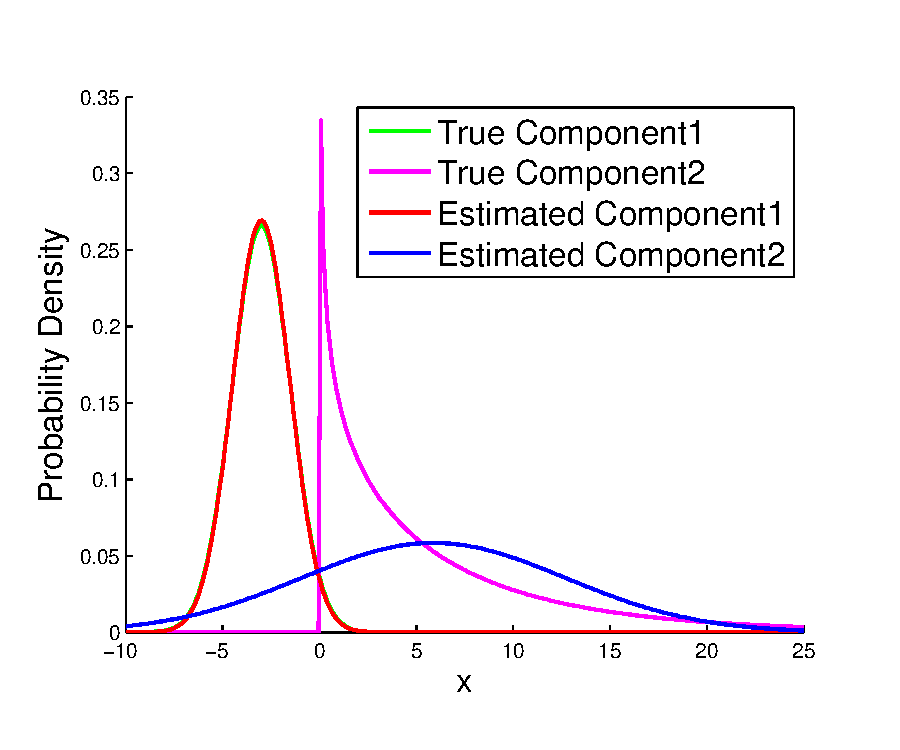
\includegraphics[width=0.65\columnwidth]{../experiment/visualization/em_visual_k_2_view_1-crop} \\
%   (a) EM using Mixture of Gaussians Model\\
%   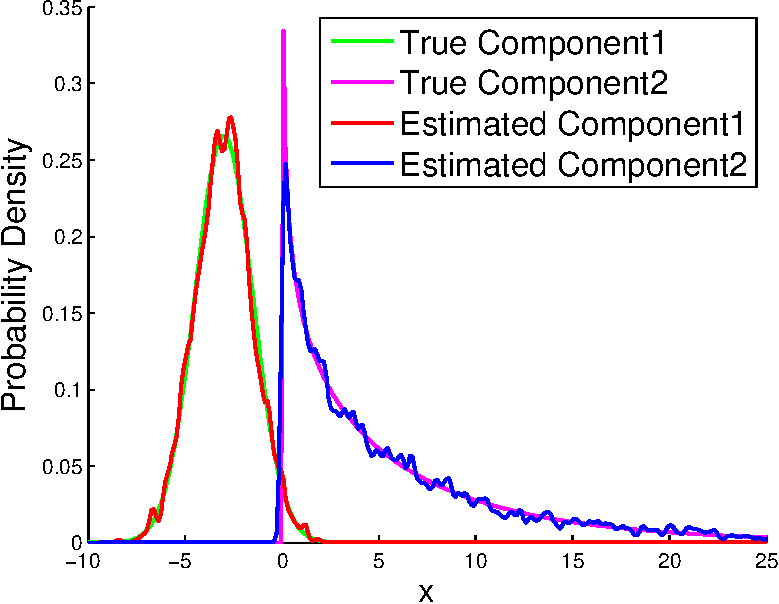
\includegraphics[width=0.65\columnwidth]{../experiment/visualization/visual_k_2_view_1-crop-crop} \\
%   (b) Kernel Spectral
%   \end{tabular}
%   \vspace{-3mm}
%   \caption{Kernel spectral algorithm is able to adapt to the shape of the mixture components, while EM algorithm for mixture of Gaussians misfit the Gamma distribution.}\label{fig:shape}
%   \vspace{-3mm}
% \end{figure}
%
%

{\bf Results.} We first illustrated the actual recovered conditional densities of our method and EM-GMM in Figure~\ref{fig:shape} as a concrete example. The kernel spectral algorithm recovers nicely both the Gaussian and Gamma components, while the EM-GMM fails to fit the Gamma component.

\begin{figure}[t]
	\vspace{-3mm}
  \subfigure[EM Gaussians Mixture]{
      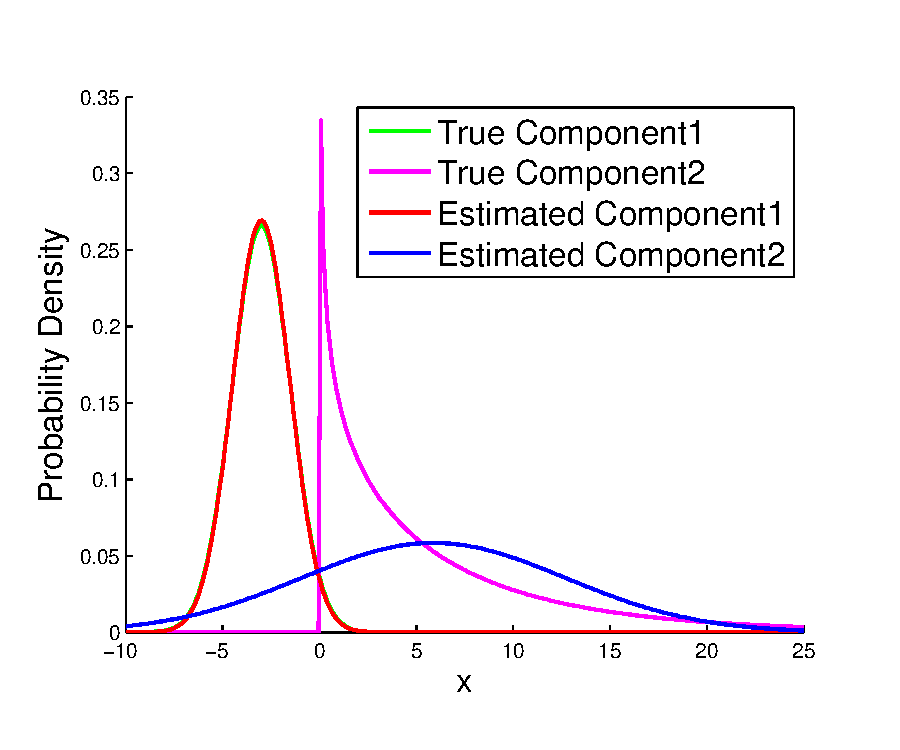
\includegraphics[width=0.47\columnwidth]{../experiment/visualization/em_visual_k_2_view_1-crop}
  }
  \subfigure[Kernel Spectral]{
      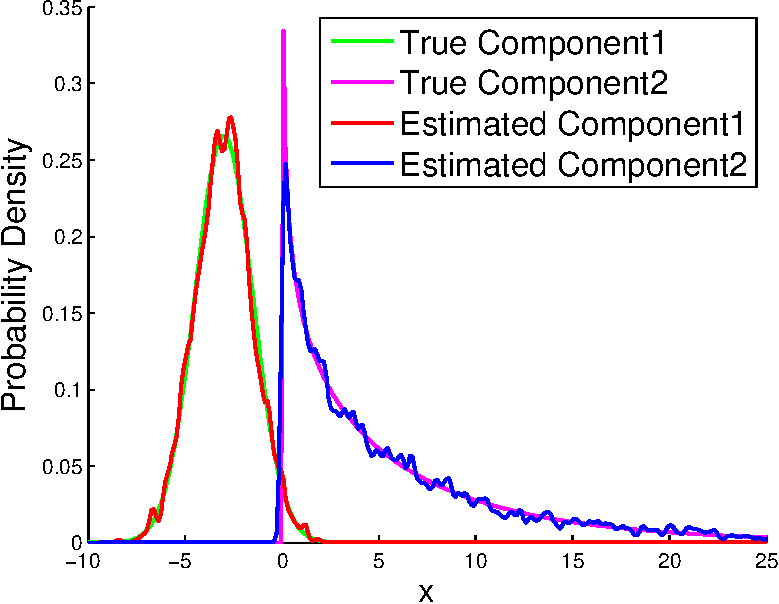
\includegraphics[width=0.47\columnwidth]{../experiment/visualization/visual_k_2_view_1-crop-crop}
  }
	\vspace{-4mm}
  \caption{Kernel spectral algorithm is able to adapt to the shape of the mixture components, while EM algorithm for mixture of Gaussians misfits the Gamma distribution.}\label{fig:shape}
	\vspace{-3mm}
\end{figure}

More quantitative results are plotted in Figure~\ref{fig:synthetic}. It is clear that the kernel spectral method converges rapidly with the data increment in all experiment settings. In the mixture of Gaussians setting, the EM algorithm is best since the model is correctly specified. The spectral algorithm for spherical Gaussians does not perform well since the assumption of the method is too restricted. The performance of our kernel method converges to that of the EM algorithm. In the mixture of Gaussian and Gamma setting, our kernel spectral algorithm achieves superior results compared to other algorithms. These results demonstrate that our algorithm is able to automatically adapt to the shape of the density.

It is worth noting that both the discretized spectral algorithm and nonparametric EM-like algorithm did not perform as well. In the discretized spectral method, the joint distribution is estimated by histogram. It is well-known that the histogram estimation suffers from poor performance even for 3 dimensional data. In the nonparametric EM-like algorithm, besides the issue of local minima, its performance also highly depends on the initialization. And the flexibility of nonparametric densities without regularization makes the issue of overfitting quite severe, often leading to a single component in the algorithm.

%We also note that the performance of EM GMM degrades as the number of components increases, and our method outperforms EM in higher dimensions.
We also note that the our method outperforms the EM-GMM more as the number of components increases.
This is the key advantage of our method in that it has favorable performance in higher dimensions, which agrees with the theoretical result in Theorem~\ref{thm:samplebound} that the sample complexity depends only quadratically in the number of components, when other parameters are held fixed.

% \begin{figure*}[!t]
% %   \centering
%   \hspace{-7mm}
%   \renewcommand{\tabcolsep}{1pt}
%   \begin{tabular}{cccc}
%     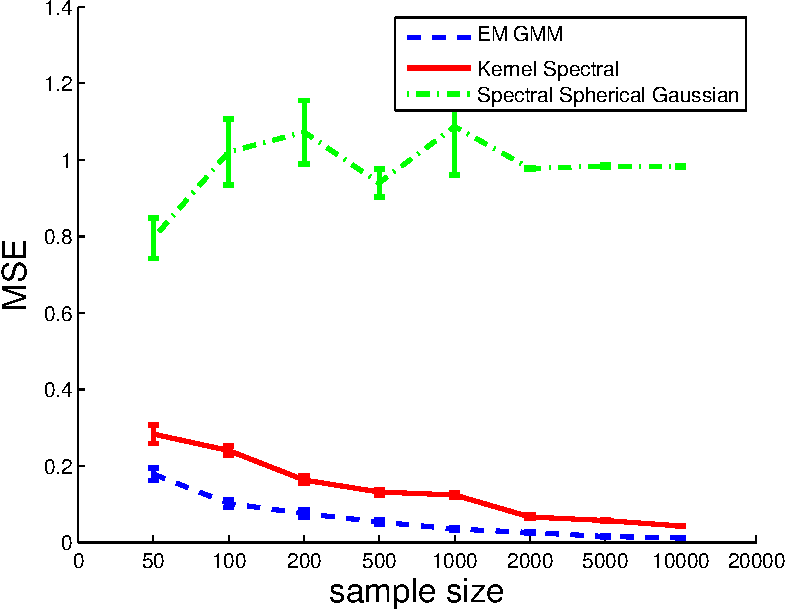
\includegraphics[width=0.26\textwidth]{../experiment/figure/sp_diff_gauss_k_2_view_1-crop} &
%     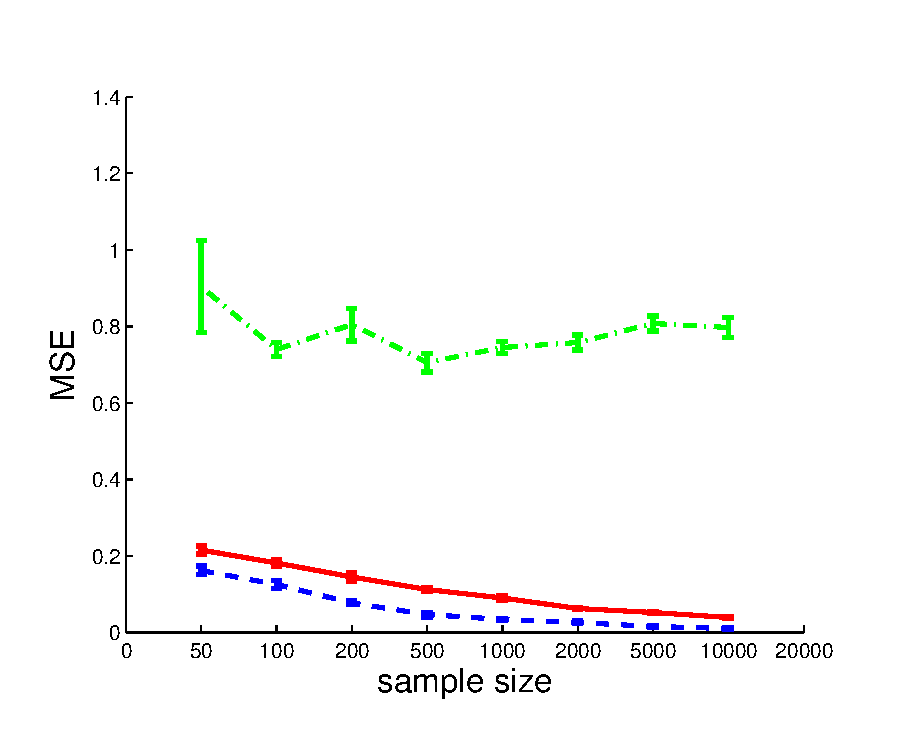
\includegraphics[width=0.26\textwidth]{../experiment/figure/sp_diff_gauss_k_3_view_1-crop} &
%     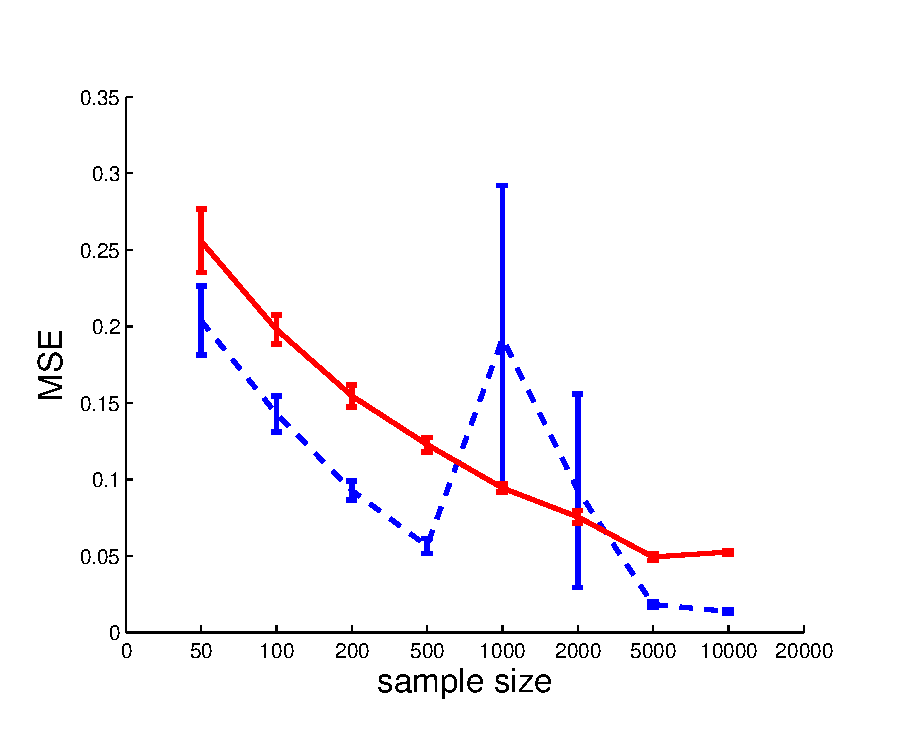
\includegraphics[width=0.26\textwidth]{../experiment/figure/sp_diff_gauss_k_4_view_1-crop} &
%     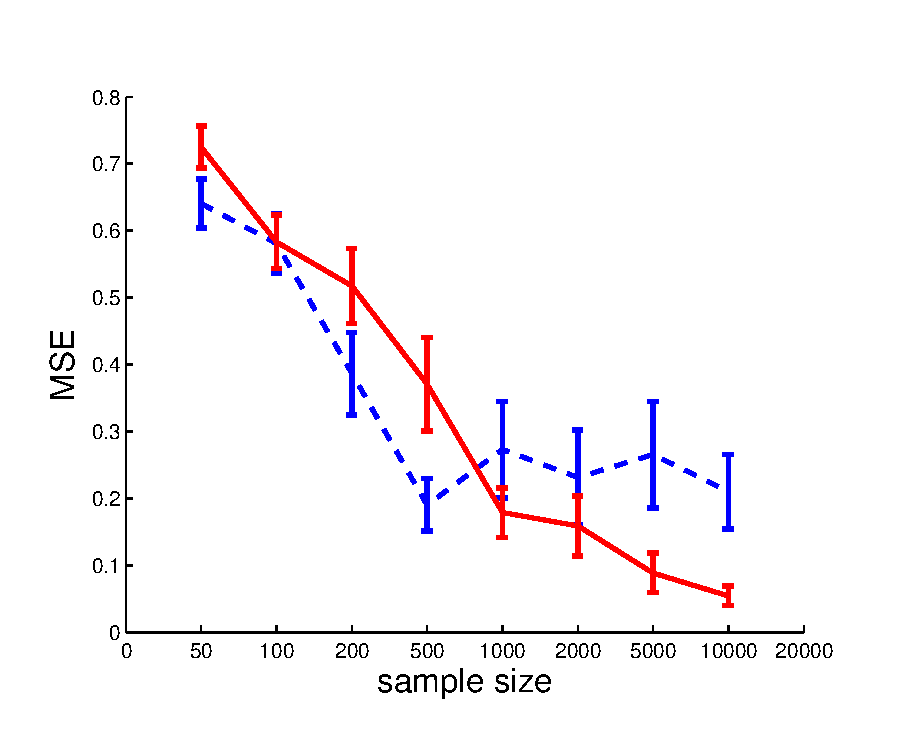
\includegraphics[width=0.26\textwidth]{../experiment/figure/sp_diff_gauss_k_8_view_1-crop} \\
%     (a) Gaussian $k=2$ & (b) Gaussian $k=3$ & (c) Gaussian $k=4$ & (d) Gaussian $k=8$ \\
%     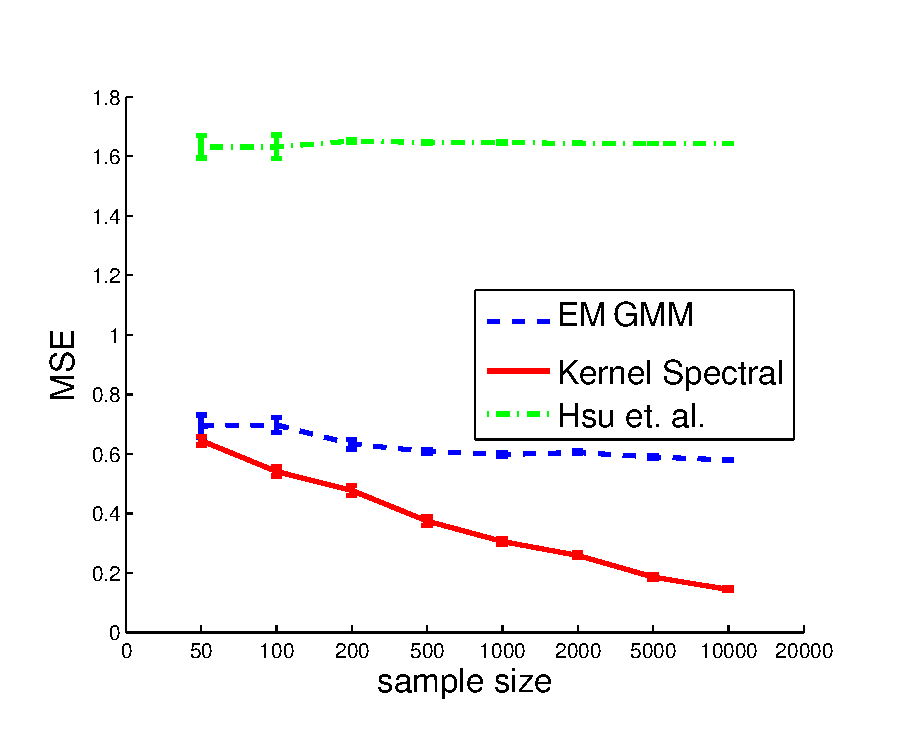
\includegraphics[width=0.26\textwidth]{../experiment/figure/sp_diff_heter_k_2_view_3-crop} &
%     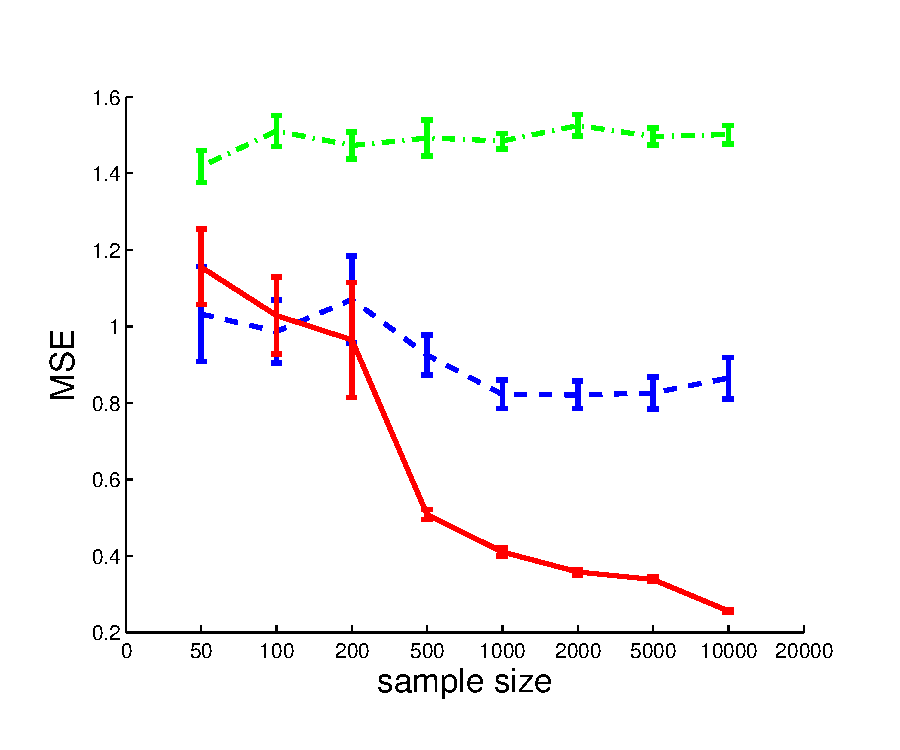
\includegraphics[width=0.26\textwidth]{../experiment/figure/sp_diff_heter_k_3_view_3-crop} &
%     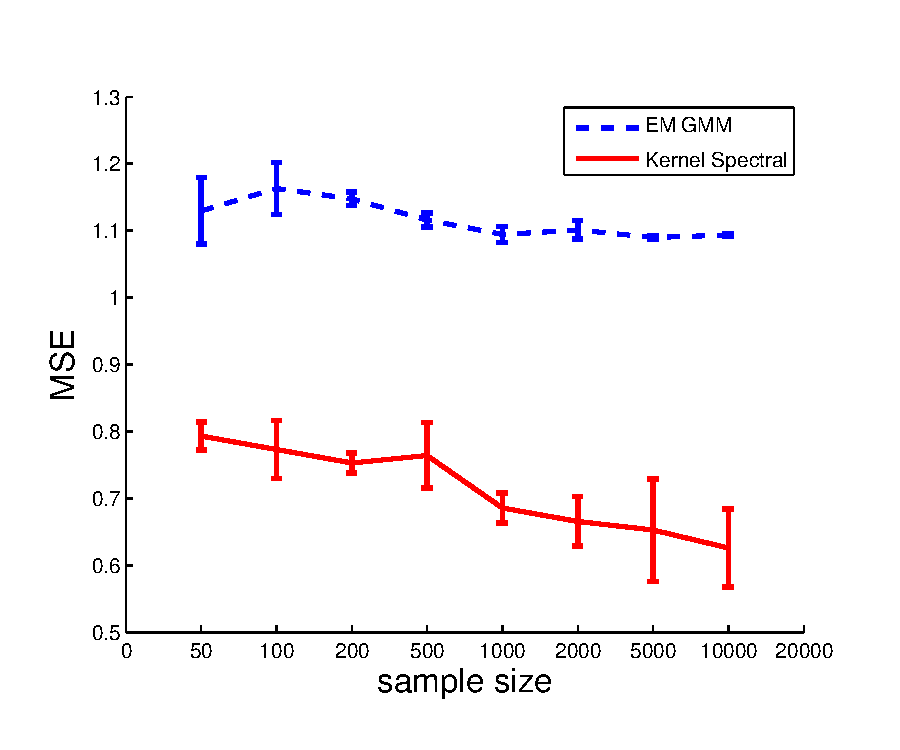
\includegraphics[width=0.26\textwidth]{../experiment/figure/sp_diff_heter_k_4_view_1-crop} &
%     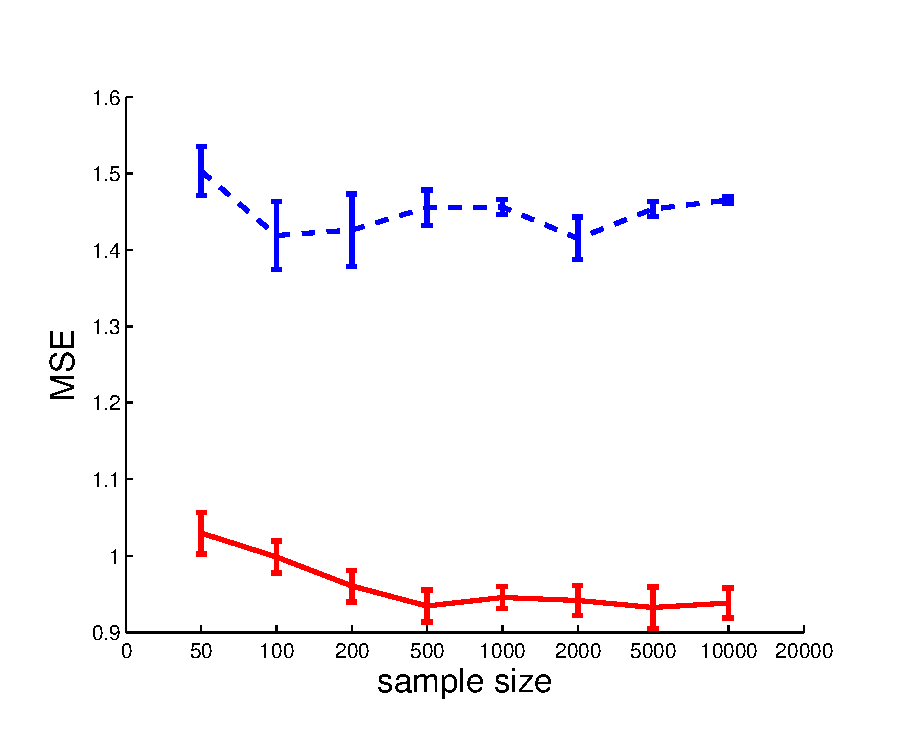
\includegraphics[width=0.26\textwidth]{../experiment/figure/sp_diff_heter_k_8_view_2-crop} \\
%     (e) Gaussian/Gamma $k=2$ & (f) Gaussian/Gamma $k=3$ & (g) Gaussian/Gamma $k=4$ & (h) Gaussian/Gamma $k=8$ \\
%   \end{tabular}
%   \vspace{-3mm}
%   \caption{(a)-(d) Mixture of Gaussian distributions with $k=2,3,4,8$ components. (e)-(h) Mixture of Gaussian/Gamma distribution with $k=2,3,4,8$. For the former case, the performance of kernel spectral algorithm converge to those of EM algorithm for mixture of Gaussian model. For the latter case, the performance of kernel spectral algorithm are consistently much better than EM algorithm for mixture of Gaussian model. Spherical Gaussian spectral algorithm does not work for $k=4,8$, and hence not plotted.}\label{fig:synthetic}
%   \vspace{-3mm}
% \end{figure*}

\begin{figure*}[!t]
  \centering
  \hspace{-6mm}
  \renewcommand{\tabcolsep}{1pt}
  \begin{tabular}{cccc}
    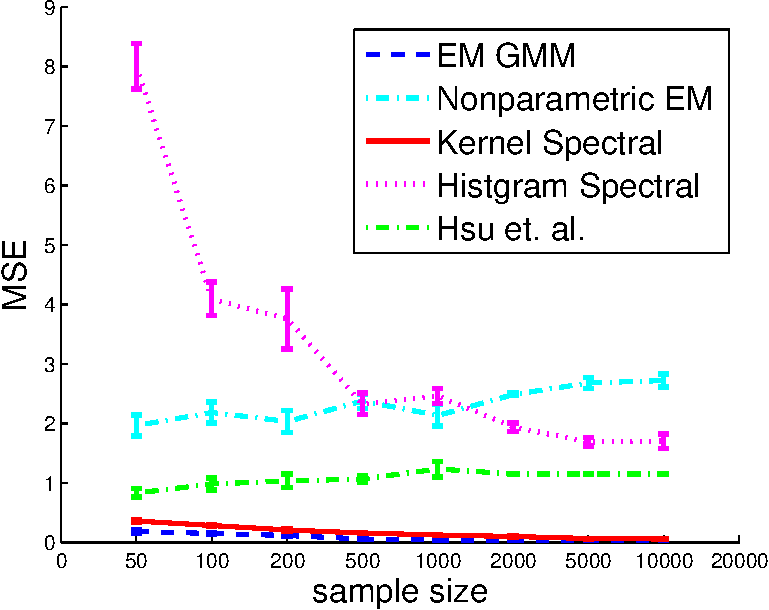
\includegraphics[width=0.24\textwidth]{../experiment/figure_new/sp_diff_gauss_k_2_view_2-crop} &
    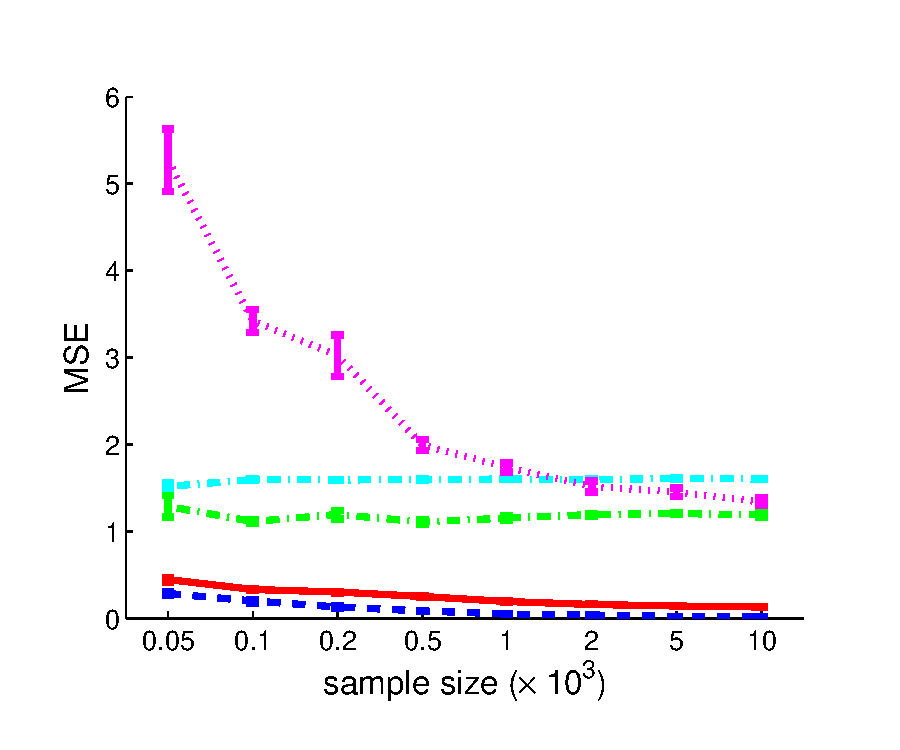
\includegraphics[width=0.24\textwidth]{../experiment/figure_new/sp_diff_gauss_k_3_view_3-crop} &
    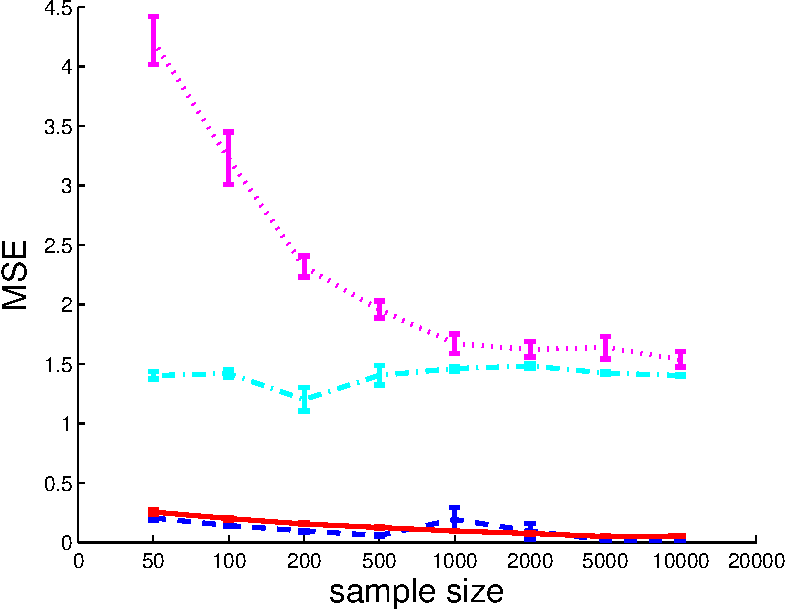
\includegraphics[width=0.24\textwidth]{../experiment/figure_new/sp_diff_gauss_k_4_view_1-crop} &
    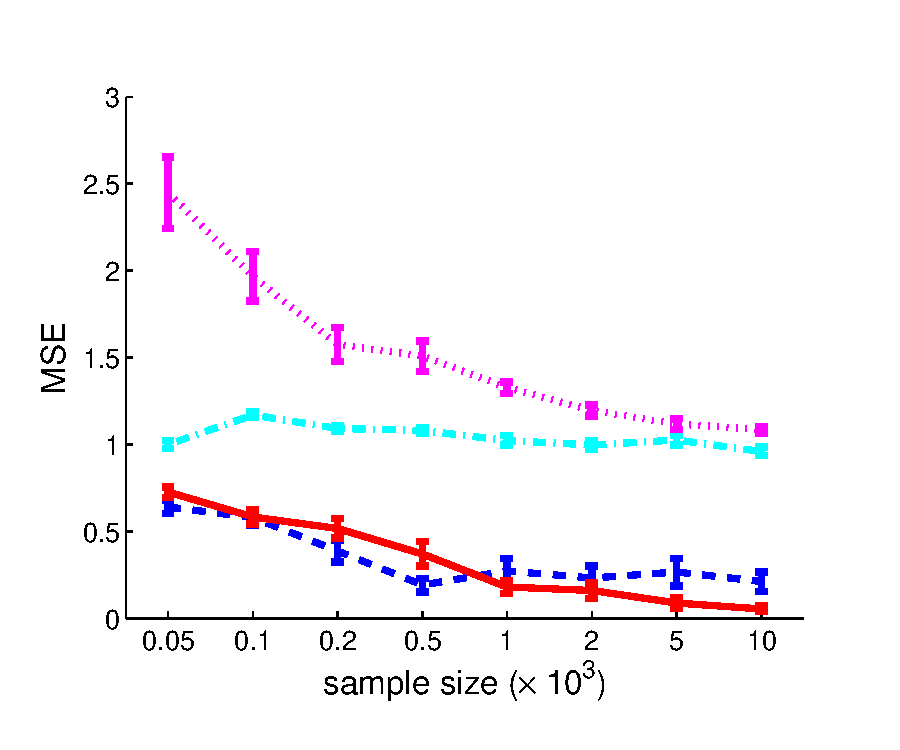
\includegraphics[width=0.24\textwidth]{../experiment/figure_new/sp_diff_gauss_k_8_view_1-crop} \\[-1mm]
    (a) Gaussian $k=2$ & (b) Gaussian $k=3$ & (c) Gaussian $k=4$ & (d) Gaussian $k=8$ \\[-1mm]
    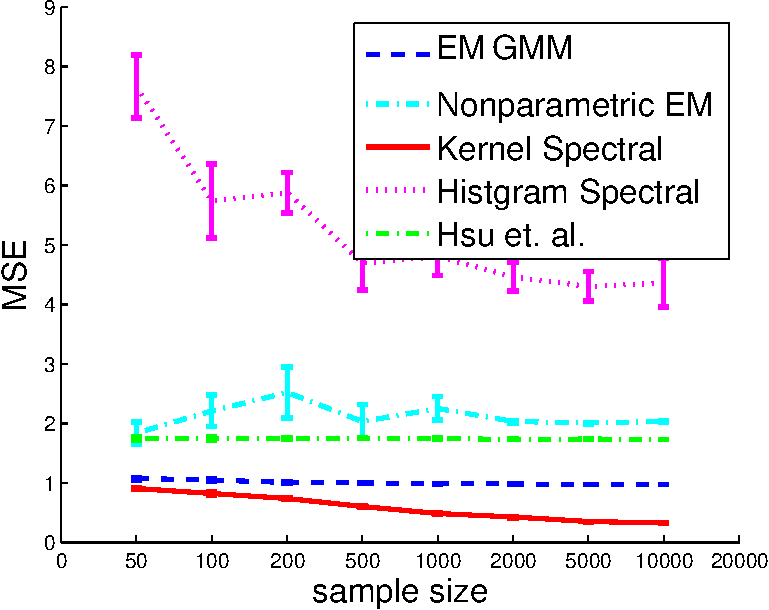
\includegraphics[width=0.24\textwidth]{../experiment/figure_new/sp_diff_heter_k_2_view_2-crop} &
    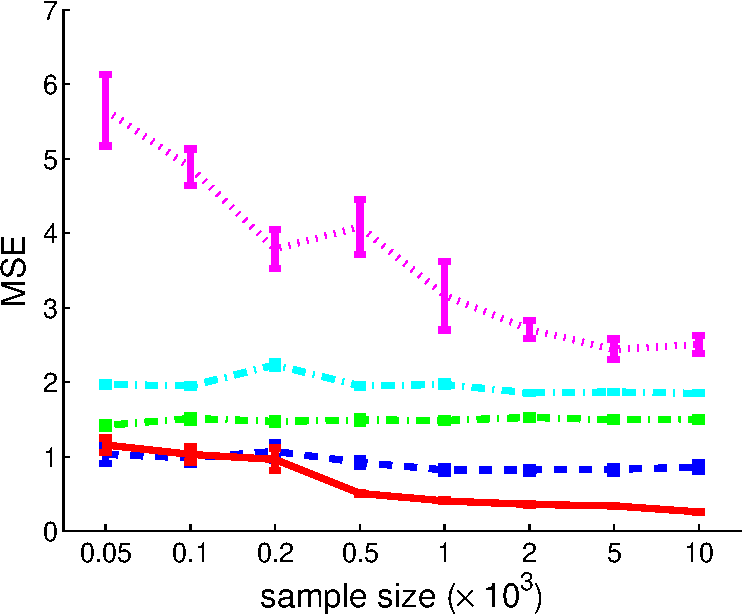
\includegraphics[width=0.24\textwidth]{../experiment/figure_new/sp_diff_heter_k_3_view_3-crop} &
    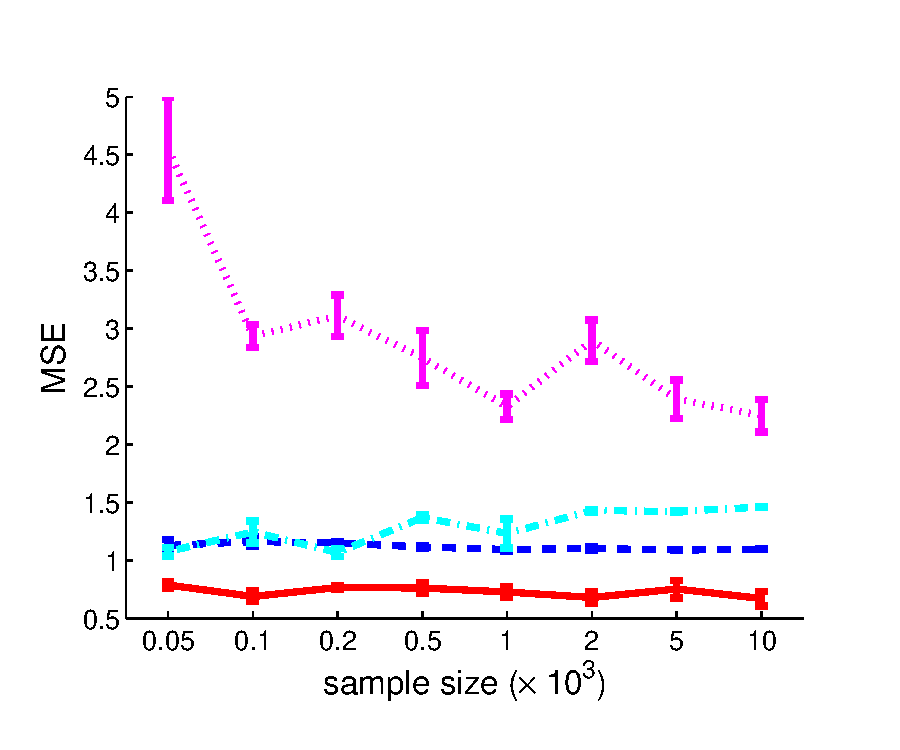
\includegraphics[width=0.24\textwidth]{../experiment/figure_new/sp_diff_heter_k_4_view_1-crop} &
    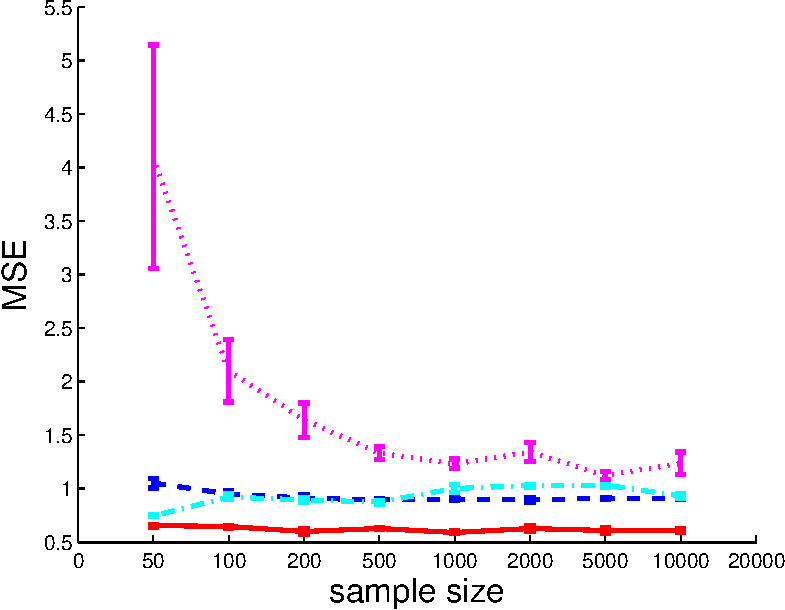
\includegraphics[width=0.24\textwidth]{../experiment/figure_new/sp_diff_heter_k_8_view_1-crop} \\[-1mm]
    (e) Gaussian/Gamma $k=2$ & (f) Gaussian/Gamma $k=3$ & (g) Gaussian/Gamma $k=4$ & (h) Gaussian/Gamma $k=8$ \\[-1mm]
  \end{tabular}
  \vspace{-2mm}
  \caption{(a)-(d) Mixture of Gaussian distributions with $k=2,3,4,8$ components. (e)-(h) Mixture of Gaussian/Gamma distribution with $k=2,3,4,8$. For the former case, the performances of kernel spectral algorithm converge to those of EM algorithm for mixture of Gaussian model. For the latter case, the performances of kernel spectral algorithm are consistently much better than EM algorithm for mixture of Gaussian model. Spherical Gaussian spectral algorithm does not work for $k=4,8$ since $k > l(=3)$ causes rank deficiency.}\label{fig:synthetic}
  \vspace{-3mm}
\end{figure*}

\begin{figure*}[t!]
  \centering
	\begin{tabular}{c}
		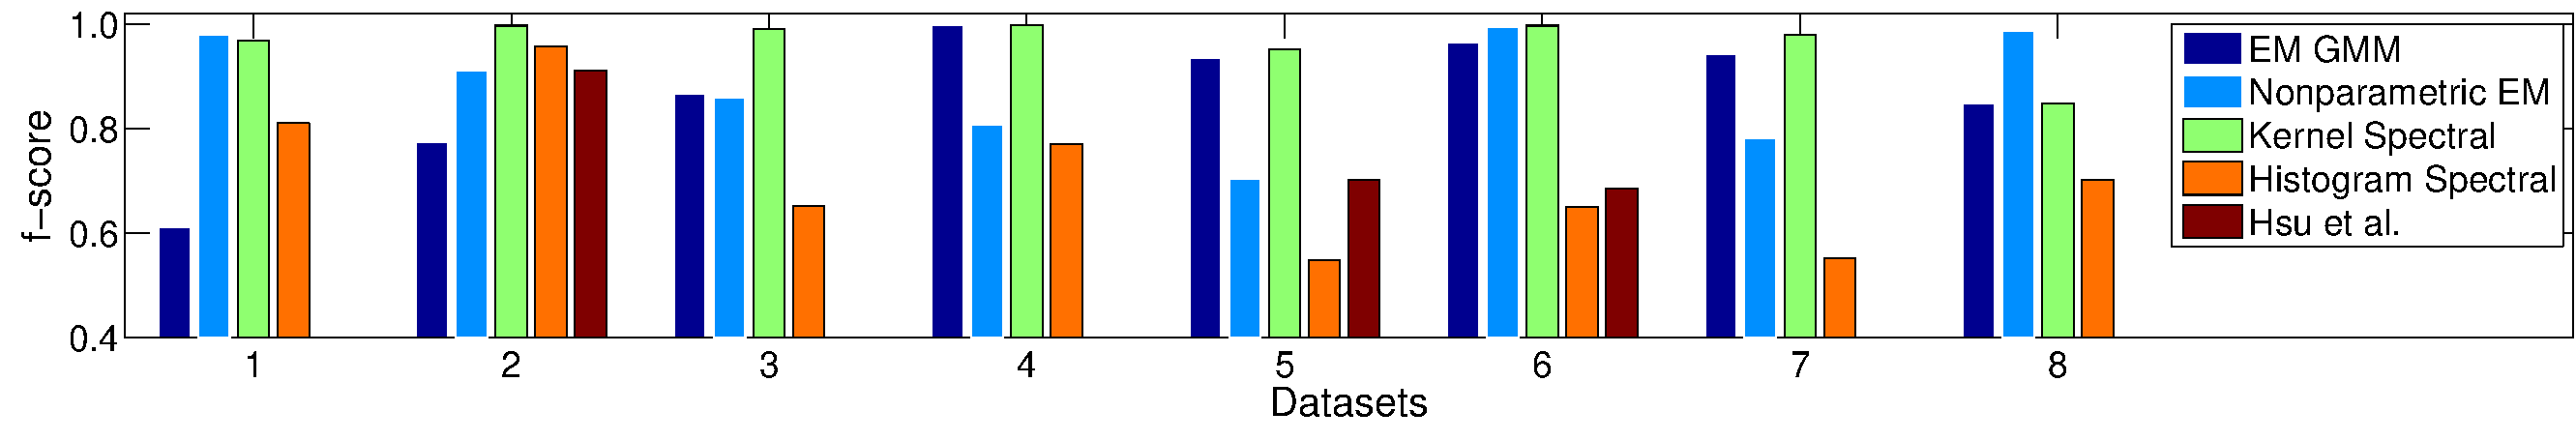
\includegraphics[width=0.82\textwidth]{../experiment/figure_new/paired_bar_chat_k_2} \\[-2mm]
		(a) number of clusters $k=2$ \\[-1mm]
		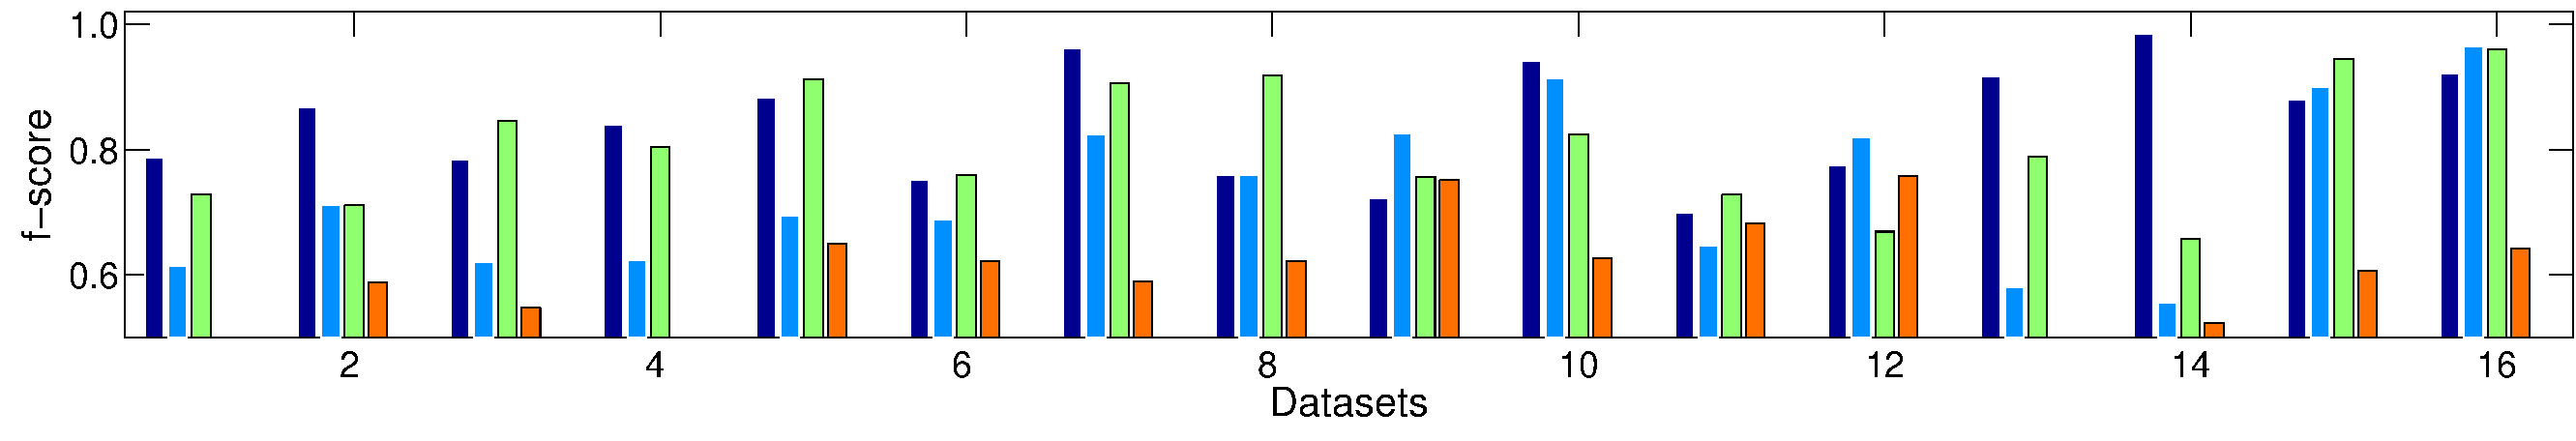
\includegraphics[width=0.98\textwidth]{../experiment/figure_new/paired_bar_chat_k_3}  \\[-2mm]
		(b) number of clusters $k=3$
	\end{tabular}
  \vspace{-4mm}
  \caption{Clustering results on the datasets from the DLBCL flow cytometry data. The results for spherical Gaussian spectral algorithm (Hsu et al.) are not plotted for datasets on which it has rank deficiency problem. The datasets are ordered by increasing sample size.}\label{fig:real_data}
  \vspace{-3mm}
\end{figure*}

\vspace{-3mm}
\subsection{Flow Cytometry Data}
\vspace{-2mm}
% 
Flow cytometry (FCM) data are multivariate measurements from flow cytometers that record light scatter and fluorescence emission properties of hundreds of thousands of individual cells. They are important to studying the cell structures of normal and abnormal cells and diagnosing human disease \cite{cytometry_nature}. This is a challenging dataset for clustering because the distribution of the data is non-Gaussian and heavily skewed.

We experimented on DLBCL dataset from the FlowCAP challenge \cite{cytometry_nature}. It contains 30 samples, and each sample consists of tens of thousands of cells measurements in 5 dimensions, with 2 to 4 clusters. Each sample is a separate clustering task, and the performance is evaluated by the weighted f-score used in \cite{cytometry_nature}. For each sample, we selected the best kernel bandwidth by log-likelihood with 5-fold cross validation. For comparison, we also evaluated the performance of EM algorithm for mixture of Gaussians with diagonal covariances. Fig.~\ref{fig:real_data} presents the results sorted by sample size.


\begin{figure}[h]
  \centering
  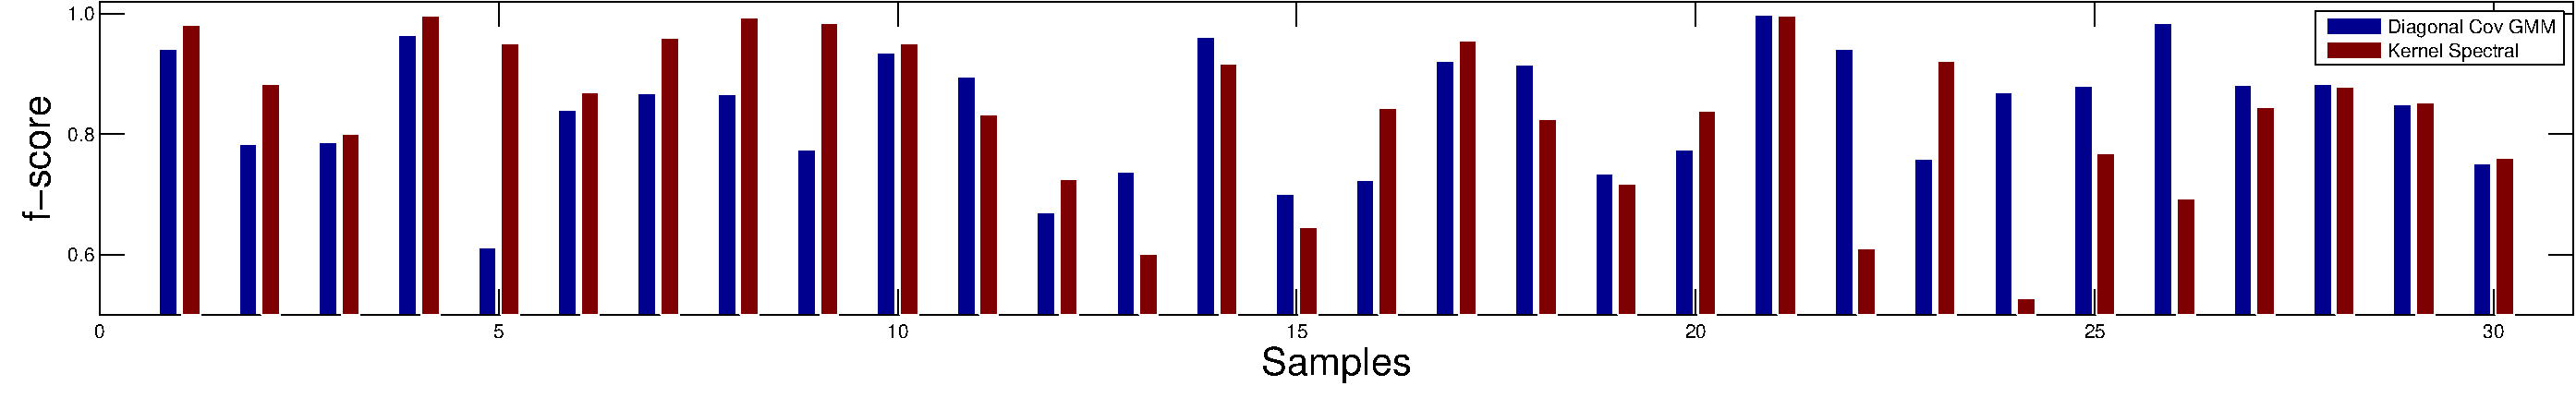
\includegraphics[width=0.9\columnwidth]{../experiment/figure/paired_bar_chat} 
   \vspace{-3mm}
  \caption{Clustering results on DLBCL flow cytometry data. There are 30 samples, each group consists of f-scores from mixture of Gaussian with diagonal covariances and kernel spectral method. The samples are ordered by increasing sample size.}\label{fig:real_data}
  \vspace{-3mm}
\end{figure}

Flow cytometry (FCM) data are multivariate measurements from flow cytometers that record light scatter and fluorescence emission properties of hundreds of thousands of individual cells. They are important to the studying of the cell structures of normal and abnormal cells and the diagnosis of human diseases. \citet{AghFinEtal13} introduced the FlowCAP-challenge whose main task is grouping the flow cytometry data automatically. Clustering on the FCM data is a difficult task because the distribution of the data is non-Gaussian and heavily skewed. We use the DLBCL Lymphoma dataset collection from~\cite{AghFinEtal13} to compare our kernel algorithm with the four alternatives.
This collection contains 24 datasets with two or three clusters, and each dataset consists of tens of thousands of cell measurements in 5 dimensions. Each dataset is a separate clustering task, so we fit a multi-view model to each dataset separately and use the maximum-a-posteriori assignment to obtain the cluster labels.  All the cell measurements have been manually labeled, therefore we can evaluate the clustering performance using f-score \cite{AghFinEtal13}.

We split the 5 dimensions into three views: dimension 1 and 2 as the first view, 3 and 4 the second, and 5 the third view based on correlation between views, since we would like the views to satisfy the conditional independence assumptions to ensure good performance for the kernel spectral method. For each dataset, we select the best kernel bandwidth by 5-fold cross validation using log-likelihood. Figure~\ref{fig:real_data} presents the results sorted by the number of clusters. Since the data are collapsed in most cases, the centers cannot span a subspace with enough rank. Thus, the method in \citep{HsuKak13} is not applicable. However, our method (kernel spectral) outperforms EM-GMM as well as the other algorithms in a majority of datasets. There are also datasets where kernel spectral algorithm has a large gap in performance compared to GMM. These are the datasets where the multi-view assumptions are heavily violated. For example, in some datasets, the correlation coefficient between dimensions 3 and 5 is 
as high as 0.927 given a particular cluster label, suggesting strong correlation between the two views. Obtaining improved and robust performance in these datasets will be a subject of our future study where we plan to develop even more robust kernel spectral algorithms.
% \aacomment{reviewer had asked how did we verify that multi-view assumption was violated. we should add this..multiple reviewers had asked about this experiment..reviewer also asked why \citep{HsuKak13} algo is not run for this.. can we quickly run this}

% \vspace{-3mm}
% \subsection{USPS Handwritten Digits Data}
% \vspace{-2mm}
% %
% The USPS handwritten digit data contains a total of 110,000 digit images, with 11,000 samples for each digit. Each image is grey-level with size 16 by 16 pixels. We extracted three different features from the images, all reduced to 50 dimensions through PCA: 1) raw image pixels, 2) Histogram of Gradients (HOG) features, and 3) Local Binary Patterns (LBP) features. These three features can be considered multiple views for a single image. Similar to the flow cytometry data, we used the clustering task as a way to evaluate how different methods model the multi-view latent variant structure in the data. The evaluation metric was the f-score used in the flow cytometry data and Normalized Mutual Information (NMI).
%
% The results are summarized in Table~\ref{tbl:usps}. Our kernel multi-view spectral methods achieve better clustering scores compared with two EM alternatives.

\vspace{-3mm}
\section*{\small Acknowledgement}
\vspace{-3mm}
{\small
This research was supported in part by NSF/NIH BIGDATA 1R01GM108341, NSF IIS1116886, NSF CAREER IIS1350983 and a Raytheon faculty fellowship to L. Song.
}

\clearpage
\newpage

% \bibliographystyle{icml2014}
% \bibliography{../nonparametric_mixture,../bibfile}

\begin{thebibliography}{25}
\providecommand{\natexlab}[1]{#1}
\providecommand{\url}[1]{\texttt{#1}}
\expandafter\ifx\csname urlstyle\endcsname\relax
  \providecommand{\doi}[1]{doi: #1}\else
  \providecommand{\doi}{doi: \begingroup \urlstyle{rm}\Url}\fi

\bibitem[Aghaeepour et~al.(2013)Aghaeepour, Finak, Consortium, Consortium,
  Hoos, Mosmann, Brinkman, Gottardo, and Scheuermann]{AghFinEtal13}
Aghaeepour, Nima, Finak, Greg, Consortium, The~FlowCAP, Consortium, The~DREAM,
  Hoos, Holger, Mosmann, Tim~R, Brinkman, Ryan, Gottardo, Raphael, and
  Scheuermann, Richard~H.
\newblock Critical assessment of automated flow cytometry data analysis
  techniques.
\newblock \emph{Nature Methods}, 10\penalty0 (3):\penalty0 228--238, 2013.

\bibitem[Allman et~al.(2009)Allman, Matias, and Rhodes]{AllMatRho09}
Allman, Elizabeth, Matias, Catherine, and Rhodes, John.
\newblock Identifiability of parameters in latent structure models with many
  observed variables.
\newblock \emph{The Annals of Statistics}, 37\penalty0 (6A):\penalty0
  3099--3132, 2009.

\bibitem[Anandkumar et~al.(2012{\natexlab{a}})Anandkumar, Ge, Hsu, Kakade, and
  Telgarsky]{AnandkumarEtal:tensor12}
Anandkumar, A., Ge, R., Hsu, D., Kakade, S.~M., and Telgarsky, M.
\newblock {Tensor Methods for Learning Latent Variable Models}.
\newblock \emph{Available at arXiv:1210.7559}, Oct. 2012{\natexlab{a}}.

\bibitem[Anandkumar et~al.(2013{\natexlab{a}})Anandkumar, Ge, Hsu, and
  Kakade]{AnandkumarEtal:community12}
Anandkumar, A., Ge, R., Hsu, D., and Kakade, S.~M.
\newblock {A Tensor Spectral Approach to Learning Mixed Membership Community
  Models}.
\newblock \emph{ArXiv 1302.2684}, Feb. 2013{\natexlab{a}}.

\bibitem[Anandkumar et~al.(2013{\natexlab{b}})Anandkumar, Hsu, Janzamin, and
  Kakade]{AnandkumarEtal:overcomplete13}
Anandkumar, A., Hsu, D., Janzamin, M., and Kakade, S.~M.
\newblock {When are Overcomplete Topic Models Identifiable? Uniqueness of
  Tensor Tucker Decompositions with Structured Sparsity}.
\newblock \emph{ArXiv 1308.2853}, Aug. 2013{\natexlab{b}}.

\bibitem[Anandkumar et~al.(2012{\natexlab{b}})Anandkumar, Foster, Hsu, Kakade,
  and Liu]{AnandkumarEtal:twosvd12}
Anandkumar, Animashree, Foster, Dean~P., Hsu, Daniel, Kakade, Sham~M., and Liu,
  Yi-Kai.
\newblock A spectral algorithm for latent dirichlet allocation.
\newblock \emph{Available at arXiv:1204.6703}, 2012{\natexlab{b}}.

\bibitem[Benaglia et~al.(2009)Benaglia, Chauveau, and Hunter]{BenChaHun09}
Benaglia, Tatiana, Chauveau, Didier, and Hunter, David~R.
\newblock An em-like algorithm for semi-and nonparametric estimation in
  multivariate mixtures.
\newblock \emph{Journal of Computational and Graphical Statistics}, 18\penalty0
  (2):\penalty0 505--526, 2009.

\bibitem[De~Lathauwer et~al.(2007)De~Lathauwer, Castaing, and
  Cardoso]{DeLathauwerEtal:FOOBI}
De~Lathauwer, L., Castaing, J., and Cardoso, J.-F.
\newblock Fourth-order cumulant-based blind identification of underdetermined
  mixtures.
\newblock \emph{IEEE Tran. on Signal Processing}, 55:\penalty0 2965--2973, June
  2007.

\bibitem[Dempster et~al.(1977)Dempster, Laird, and Rubin]{DemLaiRub77}
Dempster, A.~P., Laird, N.~M., and Rubin, D.~B.
\newblock Maximum likelihood from incomplete data via the {EM} algorithm.
\newblock \emph{Journal of the Royal Statistical Society B}, 39\penalty0
  (1):\penalty0 1--22, 1977.

\bibitem[Foster et~al.(2012)Foster, Rodu, and Ungar]{FosRodUng12}
Foster, D.P., Rodu, J., and Ungar, L.H.
\newblock Spectral dimensionality reduction for hmms.
\newblock \emph{Arxiv preprint arXiv:1203.6130}, 2012.

\bibitem[Hsu et~al.(2009)Hsu, Kakade, and Zhang]{HsuKakZha09}
Hsu, D., Kakade, S., and Zhang, T.
\newblock A spectral algorithm for learning hidden markov models.
\newblock In \emph{Proc.\ Annual Conf.\ Computational Learning Theory}, 2009.

\bibitem[Hsu \& Kakade(2013)Hsu and Kakade]{HsuKak13}
Hsu, Daniel and Kakade, Sham~M.
\newblock Learning mixtures of spherical gaussians: moment methods and spectral
  decompositions.
\newblock In \emph{Proceedings of the 4th conference on Innovations in
  Theoretical Computer Science}, ITCS '13, pp.\  11--20.  

\bibitem[Kasahara \& Shimotsu(2010)Kasahara and Shimotsu]{HirKat10}
Kasahara, Hiroyuki and Shimotsu, Katsumi.
\newblock Nonparametric identification of multivariate mixtures.
\newblock \emph{Journal of the Royal Statistical Society - Series B}, 2010.

\bibitem[Kolda \& Bader(2009)Kolda and Bader]{KolBad09}
Kolda, Tamara~G. and Bader, Brett~W.
\newblock Tensor decompositions and applications.
\newblock \emph{SIAM Review}, 51\penalty0 (3):\penalty0 455--500, 2009.

\bibitem[Kruskal(1977)]{Kruskal:77}
Kruskal, J.B.
\newblock {Three-way arrays: Rank and uniqueness of trilinear decompositions,
  with application to arithmetic complexity and statistics}.
\newblock \emph{Linear algebra and its applications}, 18\penalty0 (2):\penalty0
  95--138, 1977.

\bibitem[Parikh et~al.(2011)Parikh, Song, and Xing]{ParSonXin11}
Parikh, A., Song, L., and Xing, E.~P.
\newblock A spectral algorithm for latent tree graphical models.
\newblock In \emph{Proceedings of the International Conference on Machine
  Learning}, 2011.

\bibitem[Rosasco et~al.(2010)Rosasco, Belkin, and Vito]{RosBelVit2010}
Rosasco, L., Belkin, M., and Vito, E.D.
\newblock On learning with integral operators.
\newblock \emph{Journal of Machine Learning Research}, 11:\penalty0 905--934,
  2010.

\bibitem[Sch{\"o}lkopf et~al.(2004)Sch{\"o}lkopf, Tsuda, and Vert]{SchTsuVer04}
Sch{\"o}lkopf, B., Tsuda, K., and Vert, J.-P.
\newblock \emph{Kernel Methods in Computational Biology}.
\newblock MIT Press, Cambridge, MA, 2004.

\bibitem[Sgouritsa et~al.(2013)Sgouritsa, Janzing, Peters, and
  Sch\"{o}lkopf]{SgoJanPetSch13}
Sgouritsa, Eleni, Janzing, Dominik, Peters, Jonas, and Sch\"{o}lkopf, Bernhard.
\newblock Identifying finite mixtures of nonparametric product distributions
  and causal inference of confounders.
\newblock In \emph{Conference on Uncertainty on Artificial Intelligence (UAI)},
  2013.

\bibitem[Smola et~al.(2007)Smola, Gretton, Song, and
  {Sch\"olkopf}]{SmoGreSonSch07}
Smola, A.~J., Gretton, A., Song, L., and {Sch\"olkopf}, B.
\newblock A {H}ilbert space embedding for distributions.
\newblock In \emph{Proceedings of the International Conference on Algorithmic
  Learning Theory}, volume 4754, pp.\  13--31. Springer, 2007.

\bibitem[Song \& Dai(2013)Song and Dai]{SonDai13}
Song, L. and Dai, B.
\newblock Robust low rank kernel embedding of multivariate distributions.
\newblock In \emph{Neural Information Processing Systems (NIPS)}, 2013.

\bibitem[Song et~al.(2010)Song, Boots, Siddiqi, Gordon, and
  Smola]{SonBooSidGorSmo10}
Song, L., Boots, B., Siddiqi, S., Gordon, G., and Smola, A.~J.
\newblock Hilbert space embeddings of hidden markov models.
\newblock In \emph{International Conference on Machine Learning}, 2010.

\bibitem[Song et~al.(2011)Song, Parikh, and Xing]{SonParXin11}
Song, L., Parikh, A., and Xing, E.P.
\newblock Kernel embeddings of latent tree graphical models.
\newblock In \emph{Advances in Neural Information Processing Systems},
  volume~25, 2011.

\bibitem[Sriperumbudur et~al.(2008)Sriperumbudur, Gretton, Fukumizu, Lanckriet,
  and Sch{\"{o}}lkopf]{SriGreFukLanetal08}
Sriperumbudur, B., Gretton, A., Fukumizu, K., Lanckriet, G., and
  Sch{\"{o}}lkopf, B.
\newblock Injective {H}ilbert space embeddings of probability measures.
\newblock In \emph{Proc.\ Annual Conf.\ Computational Learning Theory}, pp.\
  111--122, 2008.

\bibitem[Wasserman(2006)]{Wasserman06}
Wasserman, L.
\newblock \emph{All of Nonparametric Statistics}.
\newblock Springer, 2006.

\end{thebibliography}


\clearpage
\newpage

\onecolumn

\begin{center}
{\Large Appendix}
\end{center}

%%-----------------------------------------------------------------------------------------------------------------------------------------------
\vspace{-3mm}
\section{Symmetrization}
\label{sec:symmetrization}
\vspace{-2mm}

We presented the kernel algorithm for learning the multi-view latent variable model where the views have identical conditional distributions. In this section, we will extend it to the general case where the views are different. Without loss of generality, we will consider recover the operator $\mu_{X_3|h}$ for conditional distribution $\PP(X_3|h)$. The same strategy applies to other views. The idea is to reduce the multi-view case to the identical-view case based on a method by~\cite{AnandkumarEtal:twosvd12}.
% %
% \begin{eqnarray*}
% \Ccal_{X_1 X_2} &=& \sum_{h \in [k]} \pi_h\, \mu_{X_1|h}\otimes \mu_{X_2|h}\\
% \Ccal_{X_2 X_3} &=& \sum_{h \in [k]} \pi_h\, \mu_{X_2|h}\otimes \mu_{X_3|h}\\
% \Ccal_{X_3 X_1} &=& \sum_{h \in [k]} \pi_h\, \mu_{X_3|h}\otimes \mu_{X_1|h}\\
% \Ccal_{X_1 X_2 X_3} &=& \sum_{h \in [k]} \pi_h\, \mu_{X_1|h}\otimes \mu_{X_2|h} \otimes \mu_{X_3|h}\\
% \end{eqnarray*}
% %
% Assume the conditional distribution for $\{X_1, X_2, X_3\}$ are in the \textit{RKHS} with kernels $\{\mathcal{K, L, G}\}$ respectively, with the feature mapping $\{\phi,\psi, \upsilon\}$.

Given the observations $\mathcal{D}_{X_1X_2X_3}=\{(x_1^i, x_2^i, x_3^i)\}_{i\in[m]}$ drawn \emph{i.i.d.} from a multi-view latent variable model $\mathbb{P}(X_1, X_2, X_3)$, let the kernel matrix associated with $X_1$, $X_2$ and $X_3$ be $K$, $L$ and $G$ respectively and the corresponding feature map be $\phi$, $\psi$ and $\upsilon$ respectively. Furthermore, let the corresponding feature matrix be $\widetilde \Phi=(\phi(x_1^1),\ldots,\phi(x_1^m))$, $\widetilde\Psi=(\phi(x_2^1),\ldots,\phi(x_2^m))$ and $\widetilde \Upsilon=(\phi(x_3^1),\ldots,\phi(x_3^m))$. Then, we have the empirical estimation of the second/third-order embedding as
%
\begin{align*}
&\widehat\Ccal_{X_1 X_2} = \frac{1}{m}\widetilde \Phi \widetilde \Psi^\top,~\widehat\Ccal_{X_3 X_1} = \frac{1}{m}\widetilde \Upsilon \widetilde \Phi^\top,~\widehat\Ccal_{X_2 X_3} = \frac{1}{m} \widetilde \Psi \widetilde \Upsilon^\top\\
&\widehat\Ccal_{X_1 X_2 X_3}:=
\frac{1}{m}\bm{I}_n \times_1 \widetilde \Phi \times_2 \widetilde \Psi \times_3 \widetilde \Upsilon
\end{align*}
%

Find two arbitrary matrices $\bm{A,B}\in \mathbb{R}^{k \times \infty}$, so that $\bm{A}\widehat{\mathcal{C}}_{X_1X_2}\bm{B}^\top$ is invertible. Theoretically, we could randomly select $k$ columns from $\Phi$ and $\Psi$ and set $\bm{A} = \Phi_k^\top, \bm{B} = \Psi_k^\top$. In practial, the first $k$ leading eigenvector directions of respect \emph{RKHS} works better.
% \bxcomment{Should we mention using SVD is better because it improves the conditioning number of $\bm{A}\widehat{\mathcal{C}}_{X_1X_2}\bm{B}^\top$?}
% \dbcomment{this is what the first svd in the code doing.}
%
Then, we have
%
\begin{eqnarray*}
\widetilde{\mathcal{C}}_{X_1 X_2} &=& \frac{1}{m}\widetilde \Phi_k^\top \widetilde\Phi\widetilde\Psi^\top\widetilde\Psi_k = \frac{1}{m}{K}_{nk}^\top{L}_{nk}\\
\widetilde{\mathcal{C}}_{X_3 X_1} &=& \widehat{\mathcal{C}}_{X_3X_1}\widetilde\Phi_k = \frac{1}{m}\widetilde\Upsilon{K}_{nk}\\
\widetilde{\mathcal{C}}_{X_3 X_2} &=& \widehat{\mathcal{C}}_{X_3X_2}\widetilde\Psi_k = \frac{1}{m}\widetilde\Upsilon{L}_{nk}\\
\widetilde{\mathcal{C}}_{X_1 X_2 X_3} &=&
\widehat{\mathcal{C}}_{X_1 X_2 X_3}\times_1\widetilde\Phi_k^\top
\times_2\widetilde\Psi_k^\top = \frac{1}{m} \bm{I}_n \times_1
{K}_{nk}^\top \times_2 {L}_{nk}^\top \times_3
\widetilde\Upsilon
\end{eqnarray*}
%

Based on these matrices, we could reduce to a single view
%
\begin{eqnarray*}
Pair_3 &=&
\widetilde{\mathcal{C}}_{X_3X_1}(\widetilde{\mathcal{C}}_{X_1X_2}^\top)^{-1}\widetilde{\mathcal{C}}_{X_3X_2}\\
&=&\frac{1}{m}\widetilde\Upsilon{K}_{nk}({L}_{nk}^\top{K}_{nk})^{-1}{L}_{nk}^\top\widetilde\Upsilon^\top = \frac{1}{m}\widetilde\Upsilon{H}\widetilde\Upsilon^\top
\end{eqnarray*}
where ${H} = {K}_{nk}(\mathcal{L}_{nk}^\top{K}_{nk})^{-1}{L}_{nk}^\top$.

Assume the leading $k$ eigenvectors $\nu_k$ lie in the span of the column of $\Upsilon$, i.e., $\nu_k = \Upsilon \beta_k$ where $\beta_k\in \mathbb{R}^{m\times 1}$
%
\begin{eqnarray*}
Pair_3\nu = \lambda \nu &\Rightarrow& (Pair_3)^\top Pair_3\nu = \lambda^2 \nu \\
&\Rightarrow&
\frac{1}{m^2} \widetilde\Upsilon{H}^\top\widetilde\Upsilon^\top\widetilde\Upsilon{H}\widetilde\Upsilon^\top\nu
= \lambda^2\nu \\
&\Rightarrow&
\frac{1}{m^2}\widetilde\Upsilon{H^\top GHG}\bm{\beta} =
\lambda^2 \widetilde\Upsilon\bm{\beta} \\
&\Rightarrow& \frac{1}{m^2}{GH^\top GHG}\beta
= \lambda^2{G}\beta
\end{eqnarray*}
%
Then, we symmetrize and whiten the third-order embedding
%
\begin{eqnarray}
Triple_3 = \frac{1}{m}\widetilde{\mathcal{C}}_{X_1X_2X_3} \times_1
[\widetilde{\mathcal{C}}_{X_3X_2}\widetilde{\mathcal{C}}_{X_1X_2}^{-1}]
\times_2
[\widetilde{\mathcal{C}}_{X_3X_1}\widetilde{\mathcal{C}}_{X_2X_1}^{-1}]
\end{eqnarray}
%
Plug
$\widetilde{\mathcal{C}}_{X_3X_2}\widetilde{\mathcal{C}}_{X_1X_2}^{-1} =
\widetilde\Upsilon{L}_{nk}({K}_{nk}^\top{L}_{nk})^{-1}$
and
$\widetilde{\mathcal{C}}_{X_3X_1}\widetilde{\mathcal{C}}_{X_2X_1}^{-1} =
\widetilde\Upsilon{K}_{nk}({L}_{nk}^\top{K}_{nk})^{-1}$,
we have

\begin{eqnarray*}
Triple_3  = \frac{1}{m}\bm{I}_n \times_1
\widetilde\Upsilon{L}_{nk}({K}_{nk}^\top
{L}_{nk})^{-1}{K}_{nk}^\top\\ \times_2
\widetilde\Upsilon{K}_{nk}({L}_{nk}^\top
{K}_{nk})^{-1}{L}_{nk}^\top \times_3 \Upsilon
\end{eqnarray*}

We multiply each mode with $\Upsilon \beta \widehat{S}_k^{-\frac{1}{2}}$ to
whitening the data and apply power method to decompose it
%
\begin{eqnarray*}
\widehat{\mathcal{T}} &=& Triple_3 \times_1 \widehat{S}_k^{-\frac{1}{2}}\beta^\top\widetilde\Upsilon^\top \times_2
\widehat{S}_k^{-\frac{1}{2}}\beta^\top\widetilde\Upsilon^\top \times_3 \widehat{S}_k^{-\frac{1}{2}}\beta^\top\widetilde\Upsilon^\top\\
&=& \frac{1}{m}\bm{I}_n \times_1
\widehat{S}_k^{-\frac{1}{2}}\beta^\top{G}\mathcal{L}_{nk}({K}_{nk}^\top
{L}_{nk})^{-1}{K}_{nk}^\top \times_2\\
&&\widehat{S}_k^{-\frac{1}{2}}\beta^\top{G}{K}_{nk}({L}_{nk}^\top
{K}_{nk})^{-1}{L}_{nk}^\top \times_3
\widehat{S}_k^{-\frac{1}{2}}\beta^\top{G}
\end{eqnarray*}
%

\section{Sample Complexity Analysis}

\subsection{Robust Tensor Power Method}
We recap the robust tensor power method for finding the tensor eigen-pairs, analyzed in detail in~\cite{AnandkumarEtal:community12}.

\begin{algorithm}
\caption{$\{\lambda, \Phi\}\leftarrow $TensorEigen$(T,\, \{v_i\}_{i\in [L]}, N)$}\label{alg:robustpower}
\begin{algorithmic}
\renewcommand{\algorithmicrequire}{\textbf{Input: }}
\renewcommand{\algorithmicensure}{\textbf{Output: }}
\REQUIRE Tensor $T\in \R^{k \times k \times k}$, set of $L$ initialization vectors $\{v_i\}_{i\in L}$, number of
iterations  $N$.
%\ENSURE Eigenpairs:  $\lambda$ is the vector of eigenvalues and $\Phi$ is the matrix of eigenvectors of  $T$.
\ENSURE the estimated eigenvalue/eigenvector pairs $\{\lambda, \Phi\}$, where $\lambda$ is the vector of eigenvalues and $\Phi$ is the matrix of eigenvectors.

\FOR{$i =1$ to $k$}
\FOR{$\tau = 1$ to $L$}
\STATE $\th{0}\leftarrow v_\tau$.
\FOR{$t = 1$ to $N$}
\STATE $\tilde{T}\leftarrow T$.
\FOR{$j=1$ to $i-1$ (when $i>1$)}
\IF{$|\lambda_j \inner{\th{t}^{(\tau)}, \phi_j}|>\xi$}
\STATE $\tilde{T}\leftarrow \tilde{T}- \lambda_j \phi_j^{\otimes 3}$.
\ENDIF
\ENDFOR

\STATE Compute power iteration update
$
\th{t}^{(\tau)}  :=
\frac{\tilde{T}(I, \th{t-1}^{(\tau)}, \th{t-1}^{(\tau)})}
{\|\tilde{T}(I, \th{t-1}^{(\tau)}, \th{t-1}^{(\tau)})\|}
$\ENDFOR
\ENDFOR

\STATE Let $\tau^* := \arg\max_{\tau \in L} \{ \tilde{T}(\th{N}^{(\tau)},
\th{N}^{(\tau)}, \th{N}^{(\tau)}) \}$.

\STATE Do $N$ power iteration updates starting from
$\th{N}^{(\tau^*)}$ to obtain eigenvector estimate $\phi_i$, and set $\lambda_i :=
\tilde{T}(\phi_i, \phi_i, \phi_i)$.

\ENDFOR
\RETURN the estimated eigenvalue/eigenvectors
$(\lambda, \Phi)$.

\end{algorithmic}
\end{algorithm}


We now recap the result of~\cite[Thm. 13]{AnandkumarEtal:community12} that establishes bounds on the eigen-estimates under good initialization vectors for the above procedure. 
Let $\Tcal=\sum_{i\in [k]}\lambda_i v_i$, where $v_i$ are orthonormal vectors and $\lambda_1\geq \lambda_2\geq\ldots \lambda_k$. Let $\h{\Tcal}=\Tcal+E$ be the perturbed tensor with $\|E\|\leq \epsilon_{T}$. Recall that $N$ denotes the number of iterations of the tensor power method.
We call an initialization vector $u$ to be $(\gamma, R_0)$-good  if there exists $v_i$ such that $\inner{u, v_i}> R_0$
  and $|\inner{u, v_i}| -\max_{j<i} |\inner{u,v_j}| > \gamma  |\inner{u,v_i}|$.   Choose $\gamma=1/100$.


\begin{theorem}
\label{thm:robustpower}
There exists universal constants $C_1, C_2 > 0$  such that the
following holds.
\beq\label{eqn:robustpowerconditions}
\epsilon_{T} \leq C_1 \cdot \lambda_{\min} R_0^2,
\qquad
N \geq C_2 \cdot \left( \log(k) + \log\log\left(
\frac{\lambdamax}{\epsilon_{tensor}} \right) \right)
,
\eeq Assume there is at least one good initialization vector corresponding to each $v_i$, $i\in [k]$. The parameter $\xi$ for choosing deflation vectors in each iteration of the tensor power method in Procedure~\ref{alg:robustpower}  is chosen as $\xi\geq 25 \eps$. We obtain  eigenvalue-eigenvector pairs  $(\hat\lambda_1,\hat{v}_1), (\hat\lambda_2,\hat{v}_2), \dotsc,
(\hat\lambda_k,\hat{v}_k)$ such that  there exists a permutation $\pi$ on
$[k]$ with
\[
\|v_{\pi(j)}-\hat{v}_j\| \leq 8 \epsilon/\lambda_{\pi(j)}
, \qquad
|\lambda_{\pi(j)}-\hat\lambda_j| \leq 5\epsilon , \quad \forall j \in [k]
,
\]
and
\[
\left\|
\Tcal - \sum_{j=1}^k \hat\lambda_j \hat{v}_j^{\otimes 3}
\right\| \leq 55\eps .
\]
\end{theorem}

In the sequel, we establish concentration bounds that allows us to translate the above condition on tensor perturbation~\eqref{eqn:robustpowerconditions}  to sample complexity bounds.

\subsection{Concentration Bounds}

\subsubsection{Analysis of Whitening} 

Recall that we use the covariance operator $\Ccal_{X_1 X_2}$ for whitening the 3rd order embedding $\Ccal_{X_1, X_2, X_3}$. We first analyze the perturbation in whitening when sample estimates are employed. 

Let $\h{\Ccal}_{X_1 X_2}$ denote the sample covariance operator between variables $X_1$ and $X_2$, and let \[B:=0.5(\h{\Ccal}_{X_1 X_2}+ \h{\Ccal}_{X_1 X_2}^\top)=\h{\Ucal}\h{S}\h{\Ucal}^\top\] denote the SVD.
Let $\Ucal_k$ and $S_k$ denote the restriction to top-$k$ eigen-pairs, and let $B_{k} := \Ucal_k S_k \Ucal_k^\top$. Recall that the whitening matrix is given by $\h{\Wcal}:=\h{\Ucal}_k \h{S}_k^{-1/2}$. Now $\h{\Wcal}$ whitens $B_k$, i.e. $\h{\Wcal}^\top B_{k} \h{\Wcal}=I$.

Now consider the SVD of
\[ \h{\Wcal}^\top \Ccal_{X_1 X_2} \h{\Wcal}= A D A^\top,\] and define \[\Wcal:= \h{\Wcal} AD^{-1/2}A^\top, \] and $\Wcal$ whitens $\Ccal_{X_1 X_2}$ since $\Wcal^\top  \Ccal_{X_1 X_2} W=I$.
Recall that by exchangeability assumption, 
\[ \Ccal_{X_1,X_{2}}
  = \sum_{j=1}^k \pi_j \cdot \mu_{X|j} \otimes \mu_{X|j} \tcr{+  E_{X_1 X_2}}= M \Diag(\pi) M^\top  \tcr{+E_{X_1 X_2}}, \] where the $j^{\tha}$ column of $M$, $M_j = \mu_{X|j}$.

We now establish the following perturbation bound on the whitening procedure. Recall from \eqref{eqn:deltapairs}, $ \epsilon_{pairs}:=\nbr{\Ccal_{X_1,X_{2}} - \widehat \Ccal_{X_1,X_{2}}}_{}$. Let $\sigma_1(\cdot) \geq \sigma_2(\cdot)\ldots$ denote the singular values of an operator.

\begin{lemma}[Whitening perturbation]\label{lemma:whiten} Assuming that $\epsilon_{pairs} < 0.5 \sigma_k(\Ccal_{X_1 X_2})$,
\beq \epsilon_{W}:= \|\Diag(\pi)^{1/2}M^\top(\h{\Wcal}-\Wcal)\|\leq \frac{2(2\epsilon_{pairs} \tcr{+\sigma_{k+1}(\Ccal_{X_1 X_2})})}{ \sigma_{k}(\Ccal_{X_1 X_2})}\tcr{\cdot (1+ \sigma_{k+1}(\Ccal_{X_1 X_2}))}\eeq
\end{lemma}

\paragraph{Remark: }Note that $\sigma_{k}(\Ccal_{X_1 X_2}) = \sigma_{k}^2(M)$.

\bprf The proof is along the lines of~\cite[Lemma 16]{AnandkumarEtal:community12}, but adapted to whitening using the covariance operator here.
 \begin{align*}\|\Diag(\pi)^{1/2} M^\top(\h{\Wcal}-\Wcal)\|&= 
\|\Diag(\pi)^{1/2} M^\top W(A D^{1/2} A^\top -I)\|\\ &\leq\|\Diag(\pi)^{1/2} M^\top \Wcal\| \|D^{1/2}-I\|. \end{align*} Since $\Wcal$ whitens $\Ccal_{X_1 X_2}=M \Diag(\pi) M^\top\tcr{+E}$, we have that $\|\Diag(\pi)^{1/2} M^\top \Wcal\|=1$ \tcr{or $\|\Diag(\pi)^{1/2} M^\top \Wcal\|\leq \|I-E\|^{1/2}\leq 1+ \sigma_{k+1}(\Ccal_{X_1 X_2})$}. Now we control $\|D^{1/2}-I\|$.  Let $\tl{E}:= \Ccal_{X_1,X_{2}} -B_k$, where recall that $B=0.5( \widehat \Ccal_{X_1,X_{2}}+ \h{\Ccal}_{X_1 X_2}^\top)$ and $B_k$ is its restriction to top-$k$ singular values. Thus, we have $\|\tl{E}\|_{HS} \leq \epsilon_{pairs} + \sigma_{k+1}(B)\leq 2\epsilon_{pairs}\tcr{+\sigma_{k+1}(\Ccal_{X_1 X_2})} $.
 We now have
\begin{align*}
\|D^{1/2}-I\|&\leq \|(D^{1/2}-I)(D^{1/2}+I)\|\leq \|D-I\|
\\ &=\|AD A^\top - I\| = \|\h{\Wcal}^\top \Ccal_{X_1 X_2}  \h{\Wcal} -I\|\\ &=\| \h{\Wcal}^\top  \tl{E} \h{\Wcal}\| \leq \|\h{\Wcal}\|^2 ( 2 \epsilon_{pairs}\tcr{+\sigma_{k+1}(\Ccal_{X_1 X_2})}).
\end{align*}Now
\[ \|\h{\Wcal}^2\| \leq\frac{1}{ \sigma_k(\h{\Ccal}_{X_1 X_2})}\leq \frac{2}{\sigma_k(\Ccal_{X_1 X_2})},\] when  $\epsilon_{pairs}<0.5 \sigma_k(\Ccal_{X_1 X_2})$.
\eprf

\subsubsection{Tensor Concentration Bounds}

Recall that the whitened tensor from samples is given by
$$\h{\Tcal} := \h{\Ccal}_{X_1 X_2 X_3} \times_1 (\h{\Wcal}^\top) \times_2 (\h{\Wcal}^\top) \times_3 (\h{\Wcal}^\top).$$ We want to establish its perturbation from the whitened tensor using exact statistics
$$\Tcal := \Ccal_{X_1 X_2 X_3} \times_1 (\Wcal^\top ) \times_2 (\Wcal^\top ) \times_3 (\Wcal^\top ).$$ Further, we have 
$$\Ccal_{X_1 X_2 X_3}= \sum_{h\in [k]} \pi_h \cdot \mu_{X|h} \otimes \mu_{X|h} \otimes \mu_{X|h} \tcr{+ E_{X_1, X_2, X_3}}$$

Let $\epsilon_{triples}:= \|\h{\Ccal}_{X_1 X_2 X_3}-\Ccal_{X_1 X_2 X_3}\|_{}$. Let $\pi_{\min}:=\min_{h\in [k]}\pi_h$.

\begin{lemma}[Tensor perturbation bound]
Assuming that $\epsilon_{pairs} < 0.5 \sigma_k(\Ccal_{X_1 X_2})$, we have
\beq\label{eqn:epsilonT} \epsilon_T:= \|\h{\Tcal} - \Tcal\|
\leq \frac{2\sqrt{2}\epsilon_{triples}}{\sigma_k(\Ccal_{X_1 X_2})^{1.5} }+\frac{\epsilon_W^3}{\sqrt{\pi_{\min}}}
\tcr{+ \|E_{X_1 X_2 X_3}\| \frac{\epsilon_W^3}{\pi_{\min}^{1.5} \sigma_k(M)^3} }.\eeq
\end{lemma} 


\bprf  Define
  intermediate tensor
\begin{align*} \tl{\Tcal}&:= \Ccal_{X_1 X_2 X_3} \times_1 (\h{\Wcal}^\top) \times_2 (\h{\Wcal}^\top) \times_3 (\h{\Wcal}^\top).\end{align*}
We will bound $\|\h{\Tcal}-\tl{\Tcal}\|$  and $\| \h{\Tcal}-\Tcal\|$  separately. 
\begin{align*}
\|\h{\Tcal}-\tl{\Tcal}\| &\leq \|\h{\Ccal}_{X_1, X_2, X_2} - \Ccal_{X_1, X_2, X_3}\| \|\h{\Wcal}\|^3\leq \frac{2\sqrt{2}\epsilon_{triples}}{\sigma_k(\Ccal_{X_1 X_2})^{1.5} },
\end{align*}using the bound on $\|\h{\Wcal}\|$ in Lemma~\ref{lemma:whiten}. For the other term,
first note that
\[ \Ccal_{X_1, X_2, X_3} = \sum_{h\in [k]} \pi_h \cdot M_h \otimes M_h \otimes M_h \tcr{+ E_{X_1, X_2, X_3}}, \]
 \tcr{ where $\|E_{X_1, X_2, X_3}\|$ is the residual and we need to bound this in non-parametric case.}
\begin{align*} \|\h{\Tcal}-\Tcal\|&= \| \Ccal_{X_1 X_2 X_3}\times_1 (\h{\Wcal} -\Wcal)^\top \times_2 (\h{\Wcal} -\Wcal)^\top \times_3 (\h{\Wcal}-\Wcal)^\top\| \\
&\leq \frac{ \| \Diag(\pi)^{1/2}M^\top(\h{\Wcal}-\Wcal)\|^3}{\sqrt{\pi_{\min}}}
\tcr{+ \|E_{X_1 X_2 X_3}\| \|\h{\Wcal}-\Wcal\|^3}\\
&= \frac{\epsilon_W^3}{\sqrt{\pi_{\min}}}
\tcr{+ \|E_{X_1 X_2 X_3}\| \frac{\epsilon_W^3}{\pi_{\min}^{1.5} \sigma_k(M)^3} }
\end{align*}
\eprf\\


We obtain a condition on the above perturbation $\epsilon_T$ in \eqref{eqn:epsilonT} by applying Theorem~\ref{thm:robustpower} as
$ \epsilon_T\leq C_1\lambda_{\min} R_0^2$. Here, we have $\lambda_{i} = 1/\sqrt{\pi_{i}}\geq 1$. For random initialization, we have that $R_0 \sim 1/\sqrt{k}$, with probability $1-\delta$ using $\poly(k) \poly(1/\delta)$ trials~\cite[Thm. 5.1]{AnandkumarEtal:tensor12}. Thus, we require that $ \epsilon_T  \leq \frac{C_1}{k}$. Summarizing, we require for the following conditions to hold 
\beq\epsilon_{pairs}\leq 0.5 \sigma_k(\Ccal_{X_1 X_2}), \quad \epsilon_T  \leq \frac{C_1}{k}.\eeq

\aacomment{need to substitute for $\epsilon_{pairs}$ and $\epsilon_{triples}$ and if we bound the residuals, we are done.}

\subsubsection{Concentration bounds for Empirical Operators}

Concentration results for the singular value decomposition of empirical operators.

\begin{lemma} Let $\kappa:=\sup_{x \in \Omega} k(x,x)$, and $\| \cdot\|_{}$ be the Hilbert-Schmidt norm, we have for \beq \epsilon_{pairs}:=\nbr{\Ccal_{X_1 X_2} - \widehat \Ccal_{X_1 X_2}}_{},\label{eqn:deltapairs} \eeq
\begin{eqnarray}
	\Pr \cbr{\epsilon_{pairs}  \leqslant \frac{2\sqrt{2}\kappa \sqrt{\delta}}{\sqrt{m}} } \geqslant 1-2\exp(-\delta). \label{eq:operator_concentration}
\end{eqnarray}
\end{lemma}

\begin{proof}
We will use similar arguments as in~\cite{RosBelVit2010} which deals with symmetric operator. Let $\xi_{i}$ be defined as
\begin{eqnarray}
\xi_{i}\, =\, \phi(x_t^i) \otimes \phi(x_{t'}^i) - \Ccal_{X_t,X_{t'}}.
\end{eqnarray}
It is easy to see that $\mathbb{E}[\xi_{i}] = 0$. Further, we have
\begin{eqnarray}
	\sup_{x_1,x_2} \nbr{\phi(x_1) \otimes \phi(x_2)}^{2}_{} \leqslant \kappa^{2},
\end{eqnarray}
which implies that $\nbr{\Ccal_{X_1 X_2}}_{} \leqslant \kappa$, and $\nbr{\xi_i}_{} \leqslant 2 \kappa$. The result then follows from the Hoeffding's inequality in Hilbert space.
\end{proof}

Similarly, we have the concentration bound for 3rd order embedding

\begin{lemma} Let $\kappa:=\sup_{x \in \Omega} k(x,x)$, and $\| \cdot\|_{}$ be the Hilbert-Schmidt norm, we have for \beq \epsilon_{pairs}:=\nbr{\Ccal_{X_1 X_2 X_3} - \widehat \Ccal_{X_1 X_2 X_3}}_{},\label{eqn:deltapairs} \eeq
\begin{eqnarray}
	\Pr \cbr{\epsilon_{triples}  \leqslant \frac{3\sqrt{2}\kappa \sqrt{\delta}}{\sqrt{m}} } \geqslant 1-2\exp(-\delta). \label{eq:operator_concentration2}
\end{eqnarray}
\end{lemma}


%-------------------------------------------------------------------------------------
\section{Experiment on Single Conditional Distribution}

We also did some experiments for three-dimensional synthetic data that each view has the same conditional distribution. We generated the data from two settings:
\begin{itemize}
\item[1.] Mixture of Gaussian conditional density;
\item[2.] Mixture of Gaussian and shifted Gamma conditional density.
\end{itemize}
The mixture proportion and other experiment settings are exact same as the experiment in the main text. The only difference is that the conditional densities for each view here are the identical. We use the same measure to evaluate the performance. The empirical results are plotted in Figure~\ref{fig:sym_case}.

\begin{figure*}[!t]
%   \centering
  \renewcommand{\tabcolsep}{1pt}
  \begin{tabular}{cccc}
    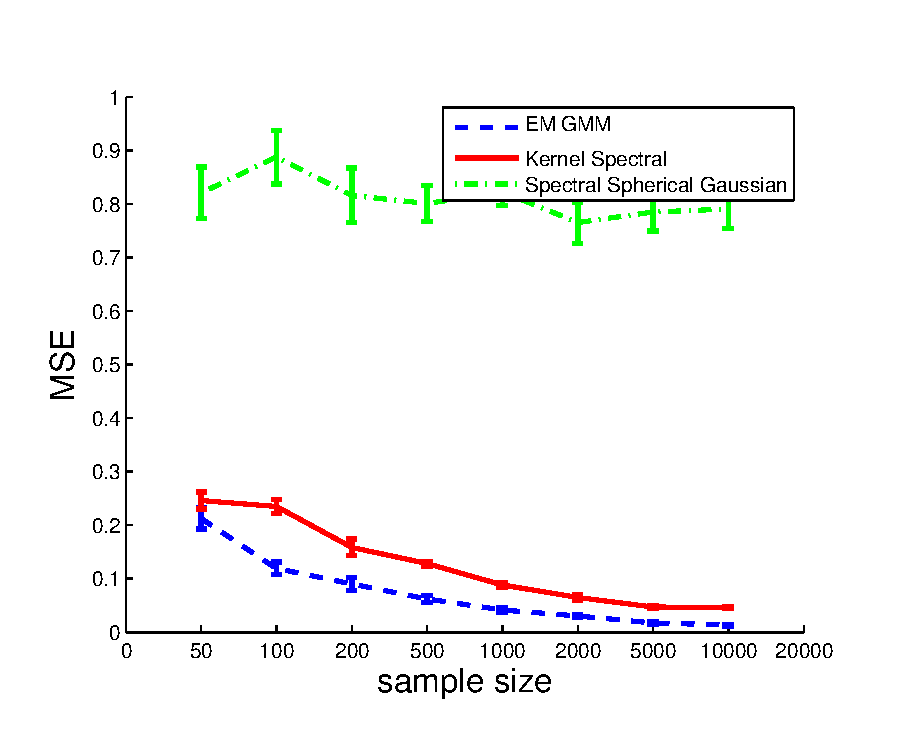
\includegraphics[width=0.26\textwidth]{../experiment/figure/sp_sym_gauss_k_2} &      
    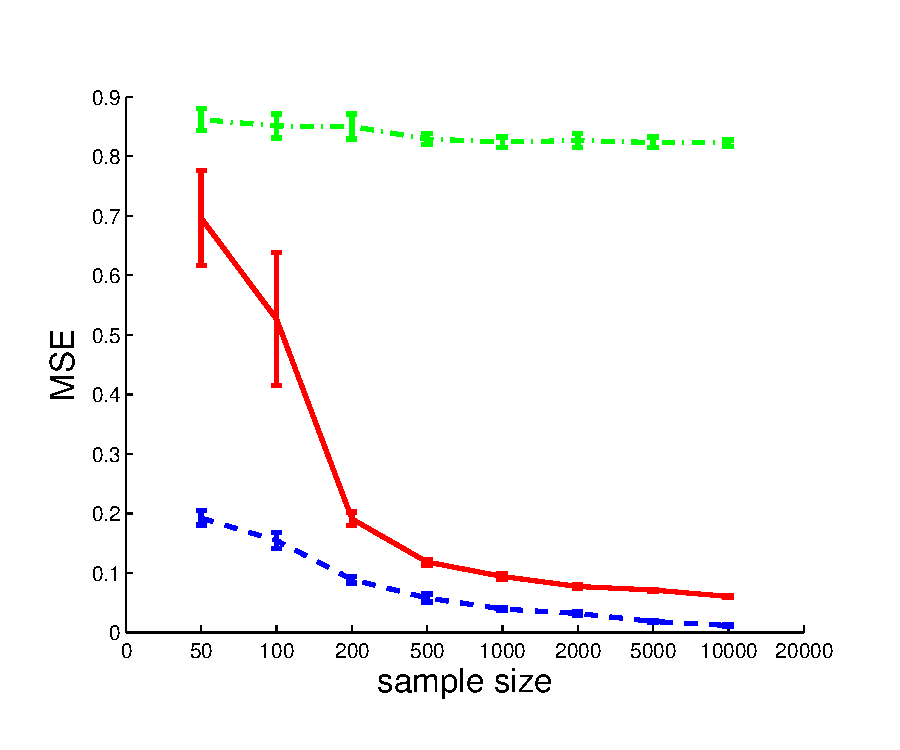
\includegraphics[width=0.26\textwidth]{../experiment/figure/sp_sym_gauss_k_3} &      
    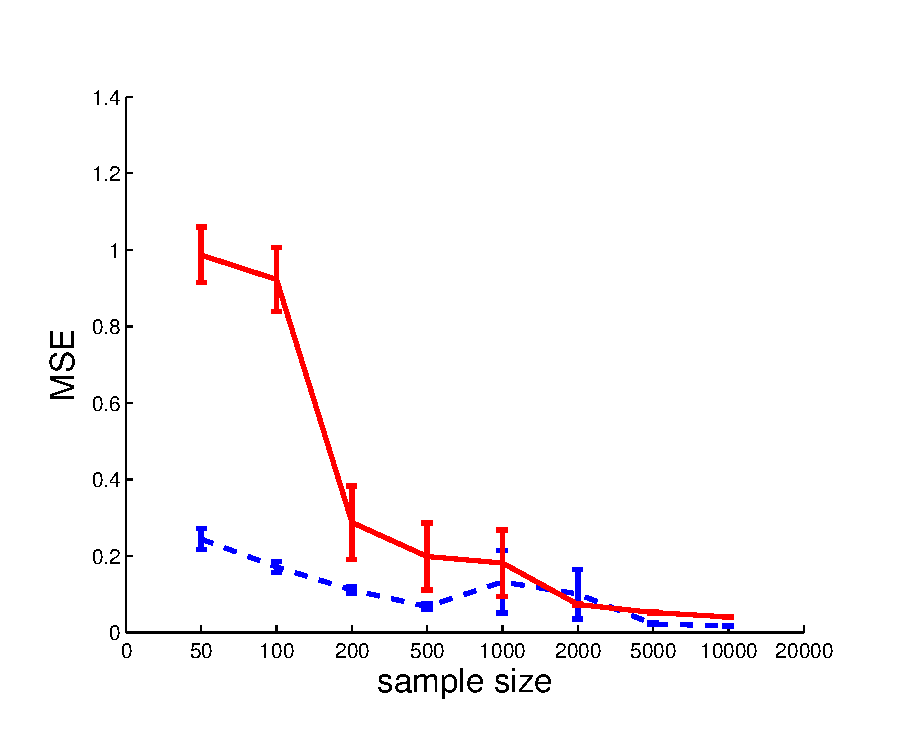
\includegraphics[width=0.26\textwidth]{../experiment/figure/sp_sym_gauss_k_4} &    
    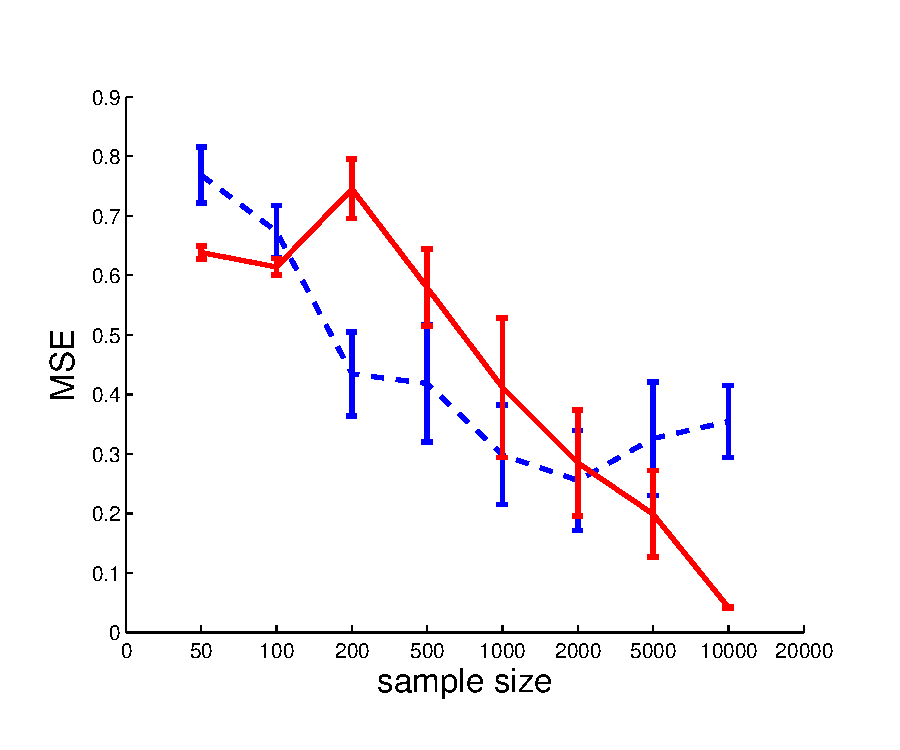
\includegraphics[width=0.26\textwidth]{../experiment/figure/sp_sym_gauss_k_8} \\    
    (a) Gaussian $k=2$ & (b) Gaussian $k=3$ & (c) Gaussian $k=4$ & (d) Gaussian $k=8$ \\ 
    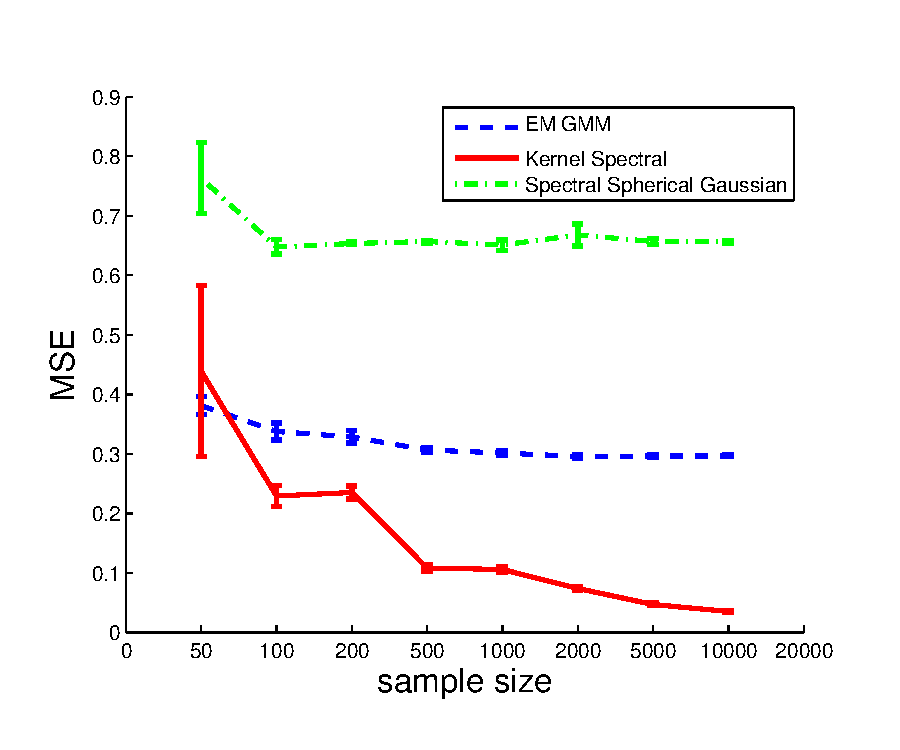
\includegraphics[width=0.26\textwidth]{../experiment/figure/sp_sym_heter_k_2} &      
    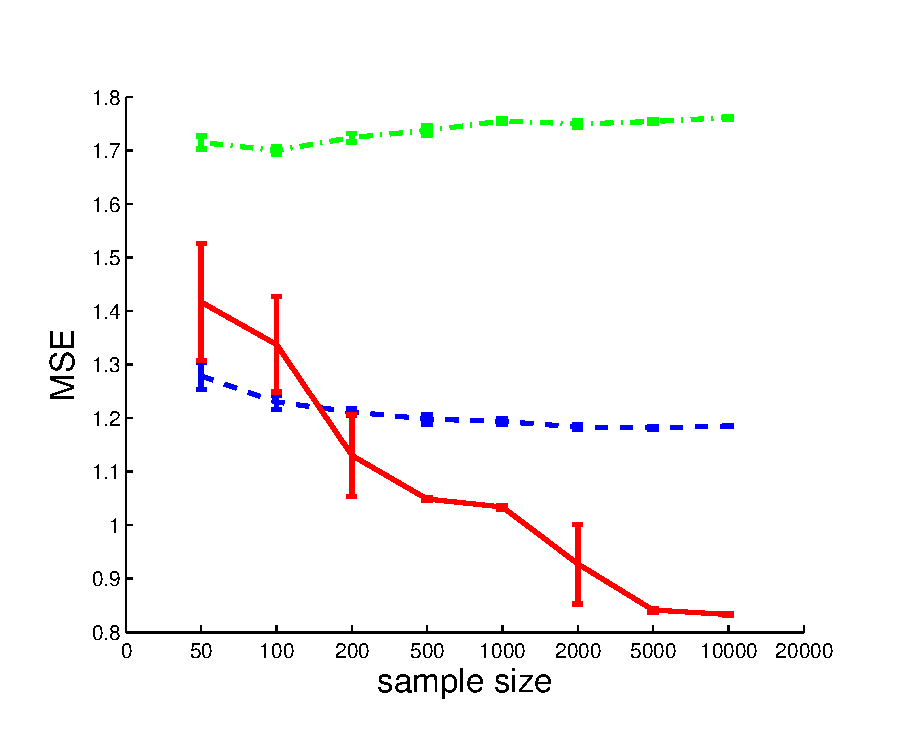
\includegraphics[width=0.26\textwidth]{../experiment/figure/sp_sym_heter_k_3} &      
    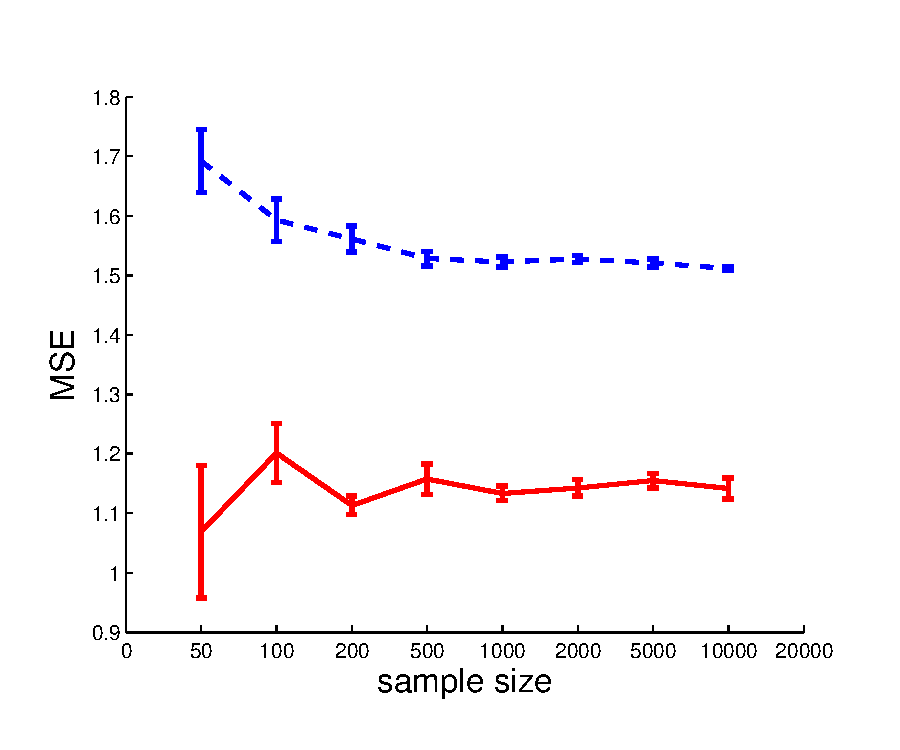
\includegraphics[width=0.26\textwidth]{../experiment/figure/sp_sym_heter_k_4} &    
    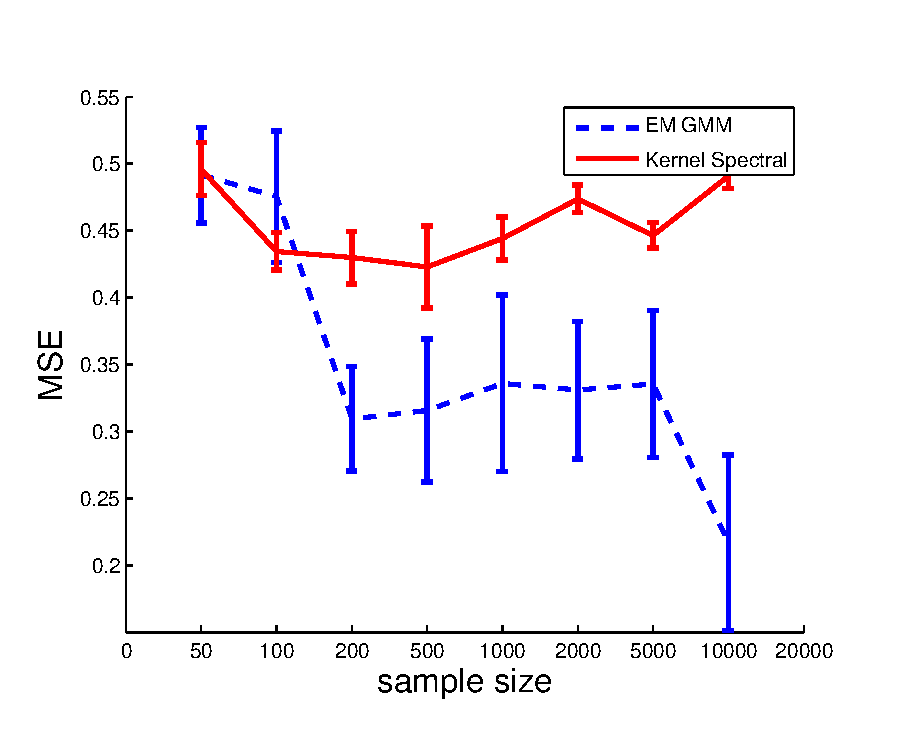
\includegraphics[width=0.26\textwidth]{../experiment/figure/sp_sym_heter_k_8} \\    
    (e) Gaussian/Gamma $k=2$ & (f) Gaussian/Gamma $k=3$ & (g) Gaussian/Gamma $k=4$ & (h) Gaussian/Gamma $k=8$ \\
  \end{tabular}
  \caption{(a)-(d) Mixture of Gaussian distributions with $k=2,3,4,8$ components. (e)-(h) Mixture of Gaussian/Gamma distribution with $k=2,3,4,8$. For the former case, the performance of kernel spectral algorithm converge to those of EM algorithm for mixture of Gaussian model. For the latter case, the performance of kernel spectral algorithm are consistently much better than EM algorithm for mixture of Gaussian model. Spherical Gaussian spectral algorithm does not work for $k=4,8$, and hence not plotted.}\label{fig:sym_case}
\end{figure*}

As we expected, the behavior of the proposed method is similar to the results in different conditional densities case. In mixture of Gaussians, our algorithm converges to the EM GMM resuls. And in the mixture of Gaussian/shift Gamma, our algorithm consistently better to other alternatives. 


% \section{Sample Complexity}
%
% Let $\rho:=\sup_{x \in \Xcal} \kappa(x,x)$,   $\| \cdot\|_{}$ be the Hilbert-Schmidt norm, $\pi_{\min}:=\min_{i\in [k]} \pi_i$ and $\sigma_k(\Ccal_{X_1X_2})$ be the $k$-th singular value of $\Ccal_{X_1X_2}$.
%
% %Assume that the mixing weights $\pi_1\geq \pi_2\ldots$ are in decreasing order.  Let $E_{X_1, X_2, X_3}$ be the residual tensor \beq\label{eqn:triplesexpression}\Ccal_{X_1 X_2 X_3}= \sum_{h\in [k]} \pi_h \cdot \mu_{X|h} \otimes \mu_{X|h} \otimes \mu_{X|h} + E_{X_1, X_2, X_3}\eeq
%
%
% \begin{theorem}[Sample Bounds]\label{thm:samplebound}
% Pick  any $\delta\in (0,1)$. When the number of samples $m$ satisfies
% \[ m >\frac{\theta\rho^2  \log\frac{2}{\delta}}{\sigma^2_k(\Ccal_{X_1 X_2})},
% \quad \theta:= \max\left(\frac{C_3 k^2}{\sigma_k( \Ccal_{X_1 X_2})}, \frac{C_4k^{2/3}\iffalse(1+\sigma_{k+1}(\Ccal_{X_1 X_2}))^2 \fi }{\pi_{\min}^{1/3}}\right),\] for some constants $C_3, C_4>0$, and the number of iterations $N$  and  the number of random initialization vectors $L$  (drawn uniformly on the sphere $\mathcal{S}^{k-1}$)  satisfy
% \begin{align*}
%   N \geq C_2 \cdot \biggl( \log(k) + \log\log\Bigl(
%  \frac{1}{\sqrt{\pi}_{\min}\epsilon_{\Tcal}} \Bigr) \biggr),
% % \sqrt{\frac{\ln(L/\log_2(k/\delta))}{\ln(k)}}
% % \cdot \Biggl( 1 - \frac{\ln(\ln(L/\log_2(k/\delta))) +
% % C_3}{4\ln(L/\log_2(k/\delta))} -
% % \sqrt{\frac{\ln(8)}{\ln(L/\log_2(k/\delta))}} \Biggr)
% % \geq 1.02 \Biggl( 1 + \sqrt{\frac{\ln(4)}{\ln(k)}}
% % \Biggr)
% % .
% \end{align*}
% for constant $C_2>0$ and  $L = \poly(k) \log(1/\delta)$,  the robust power method in~\cite{AnandkumarEtal:community12} yields eigen-pairs $(\h{\lambda}_i, \h{\phi}_i)$ such that there exists a permutation $\eta$, with probability $1-4\delta$, we have
% \begin{align*}
% &\|\pi^{-1/2}_{j} \mu_{X|h=j}-\h{\phi}_{\eta(j)}\| \leq 8 \epsilon_{\Tcal} \cdot\pi^{-1/2}_{j}
% , \\
% &|\pi^{-1/2}_{j}-\h{\lambda}_{\eta(j)}| \leq  5\epsilon_{\Tcal}, \quad \forall j \in [k]
% ,
% \end{align*}
% and
% \[
% \biggl\|
% T - \sum_{j=1}^k \hat\lambda_j \hat{\phi}_j^{\otimes 3}
% \biggr\| \leq 55\eps_{\Tcal},
% \] where $\eps_{\Tcal}$ is the tensor perturbation bound
% \begin{align*} \eps_{\Tcal} := \|\h{\Tcal} - \Tcal\| \leq&
% \frac{12 \rho \sqrt{\log\frac{2}{\delta}}}{\sqrt{m} \, \sigma_k^{1.5}(\Ccal_{X_1 X_2})} \\ &+ \frac{512 \sqrt{2} \rho^3 \left(\log\frac{2}{\delta}\right)^{1.5}}{m^{1.5} \,\sigma_k^{3}(\Ccal_{X_1 X_2}) \sqrt{\pi}_{\min}}\end{align*}
% \end{theorem}
%
% Thus, the above result provides bounds on the estimated eigen-pairs using the robust tensor power method.
% The proof is in Appendix~\ref{app:samplebound}.
%
% \paragraph{Remarks: }We note that the sample complexity is  $\poly(k, \rho, 1/\pi_{\min}, 1/\sigma_k(\Ccal_{X_1 X_2}))$ of a low order, and in particular,  it is $O(k^2)$, when the other parameters are fixed. For the special case of discrete measurements, where the kernel $\kappa(x,x')=\delta(x,x')$, we have $\rho=1$. Note that the sample complexity depends in this case only on the number of components $k$ and not on the dimensionality of the observed state space.   Thus, the robust tensor method has efficient sample and computational complexities for non-parametric latent variable estimation.

\end{document}
